\clearpage
\section{Results for the ``edge analysis'' SUS-12-019}
\label{sec:edge}

The Aachen and ETH groups have reported an excess of low-mass, opposite-sign same-flavor events (see AN 2012/200 and AN 2012/231).
In App.~\ref{sec:edge_templates} we derive predictions for the Z background in the Z mass regions for the two signal regions used for this analysis,
and use these predictions to derive an estimate of the low-mass $\gamma^*$/Z contributions using an extrapolation technique
commonly referred to as the ``$R_{out/in}$'' technique.

%In App.~\ref{sec:edge_triggers} we provide a cross-check using single lepton triggers.

\subsection{Z Background Predictions for the ``Edge Analysis''}
\label{sec:edge_templates}

The two signal regions of the edge analysis are defined as:

\begin{itemize}
\item Low-\MET signal region (ETH)
  \begin{itemize}
  \item 2 \pt $>$ 20 GeV leptons with $|\eta|<2.4$
  \item At least 3 jets (\pt\ $>$ 40 GeV, $|\eta|<3$)
  \item \MET\ $>$ 100 GeV
  \end{itemize}
\item High-\MET signal region (Aachen)
  \begin{itemize}
  \item leading lepton \pt $>$ 20 GeV, trailing lepton \pt\ $>$ 10 GeV, both with $|\eta|<2.4$
  \item At least 2 jets (\pt\ $>$ 40 GeV, $|\eta|<3$) with scalar sum $H_{T}>100$~GeV
  \item \MET\ $>$ 150 GeV
  \end{itemize}
\end{itemize}

We begin with a synchronization exercise to make sure that we can reproduce the ETH/Aachen results. In Table~\ref{tab:edgesync} we
display the yields in the Z mass regions of the 2 signal regions and compare these to results from the ETH group.
In general we are synchronized to 3\% or better in all channels. Note that for the purposes of this exercise we include an additional
dimuon trigger (HLT\_Mu17\_TkMu8) which is not yet included in the results that follow. The inclusion of this trigger adds 3 $\mu\mu$
events in both  the low \MET\ and high \MET\ signal regions.


\begin{table}[htb]
\begin{center}
\footnotesize
\caption{\label{tab:edgesync} Summary of the synchronization exercise with the ETH group with 9.2 fb$^{-1}$. 
The yields in the Z mass region ($81<m_{\ell\ell}<101$~GeV) are displayed for the low \MET\ and high \MET\ signal regions.}
\begin{tabular}{l|c|c}

\hline
\hline

low \MET\ signal region & UCSB-UCSD-FNAL & ETH \\
\hline
ee       & 125 & 123 \\
$\mu\mu$ & 166 & 164 \\
e$\mu$   & 186 & 186 \\

\hline
\hline

high \MET\ signal region & UCSB-UCSD-FNAL & ETH \\
\hline
ee       &  75 &  72 \\
$\mu\mu$ &  95 &  94 \\
e$\mu$   & 113 & 113 \\

\hline
\hline

\end{tabular}
\end{center}
\end{table}


In order to adapt the \MET\ templates method to predict the Z background in these regions, we make minor modifications
to the flavor-symmetric (FS) scaling factor $K$ and to the binning used for the \MET\ templates. The FS background 
is estimated using e$\mu$ events in data.
To improve the precision of this background estimate, the dilepton mass requirement is not applied, and we apply a scaling
factor $K$, which is the efficiency for e$\mu$ events to fall in the Z mass window,  extracted from MC.
The values of $K$ for various \MET\ intervals for the high-\MET\ region (using \pt\ $>$ (20,10) GeV leptons and at least 2 jets) 
are shown in Fig.~\ref{fig:K_incl_highmet}. 
Based on this plot we choose $K=0.13\pm0.02$ for \MET\ signal regions up to 200 GeV; for \MET\ 200-300 GeV and \MET\ $>$ 300 GeV
we inflate the uncertainty to $K=0.13\pm0.04$ and $K=0.13\pm0.05$, respectively, due to the limited statistical precision.
The values of $K$ for the low-\MET\ region (using \pt\ $>$ (20,20) GeV leptons and at least 3 jets) are shown in 
Fig.~\ref{fig:K_incl_lowmet}. 
Based on this plot we choose $K=0.14\pm0.02$ for \MET\ signal regions up to 200 GeV; for \MET\ 200-300 GeV and \MET\ $>$ 300 GeV
we inflate the uncertainty to $K=0.14\pm0.03$ and $K=0.14\pm0.07$, respectively. In addition, we change the 
jet \pt\ threshold for the \MET\ templates jet multiplicity binning from 30 to 40 GeV, and change the $H_T$ bins to
(0,80,100,150,200,250,300,5000) GeV.

\clearpage

\begin{figure}[!ht]
\begin{center}
\begin{tabular}{cc}
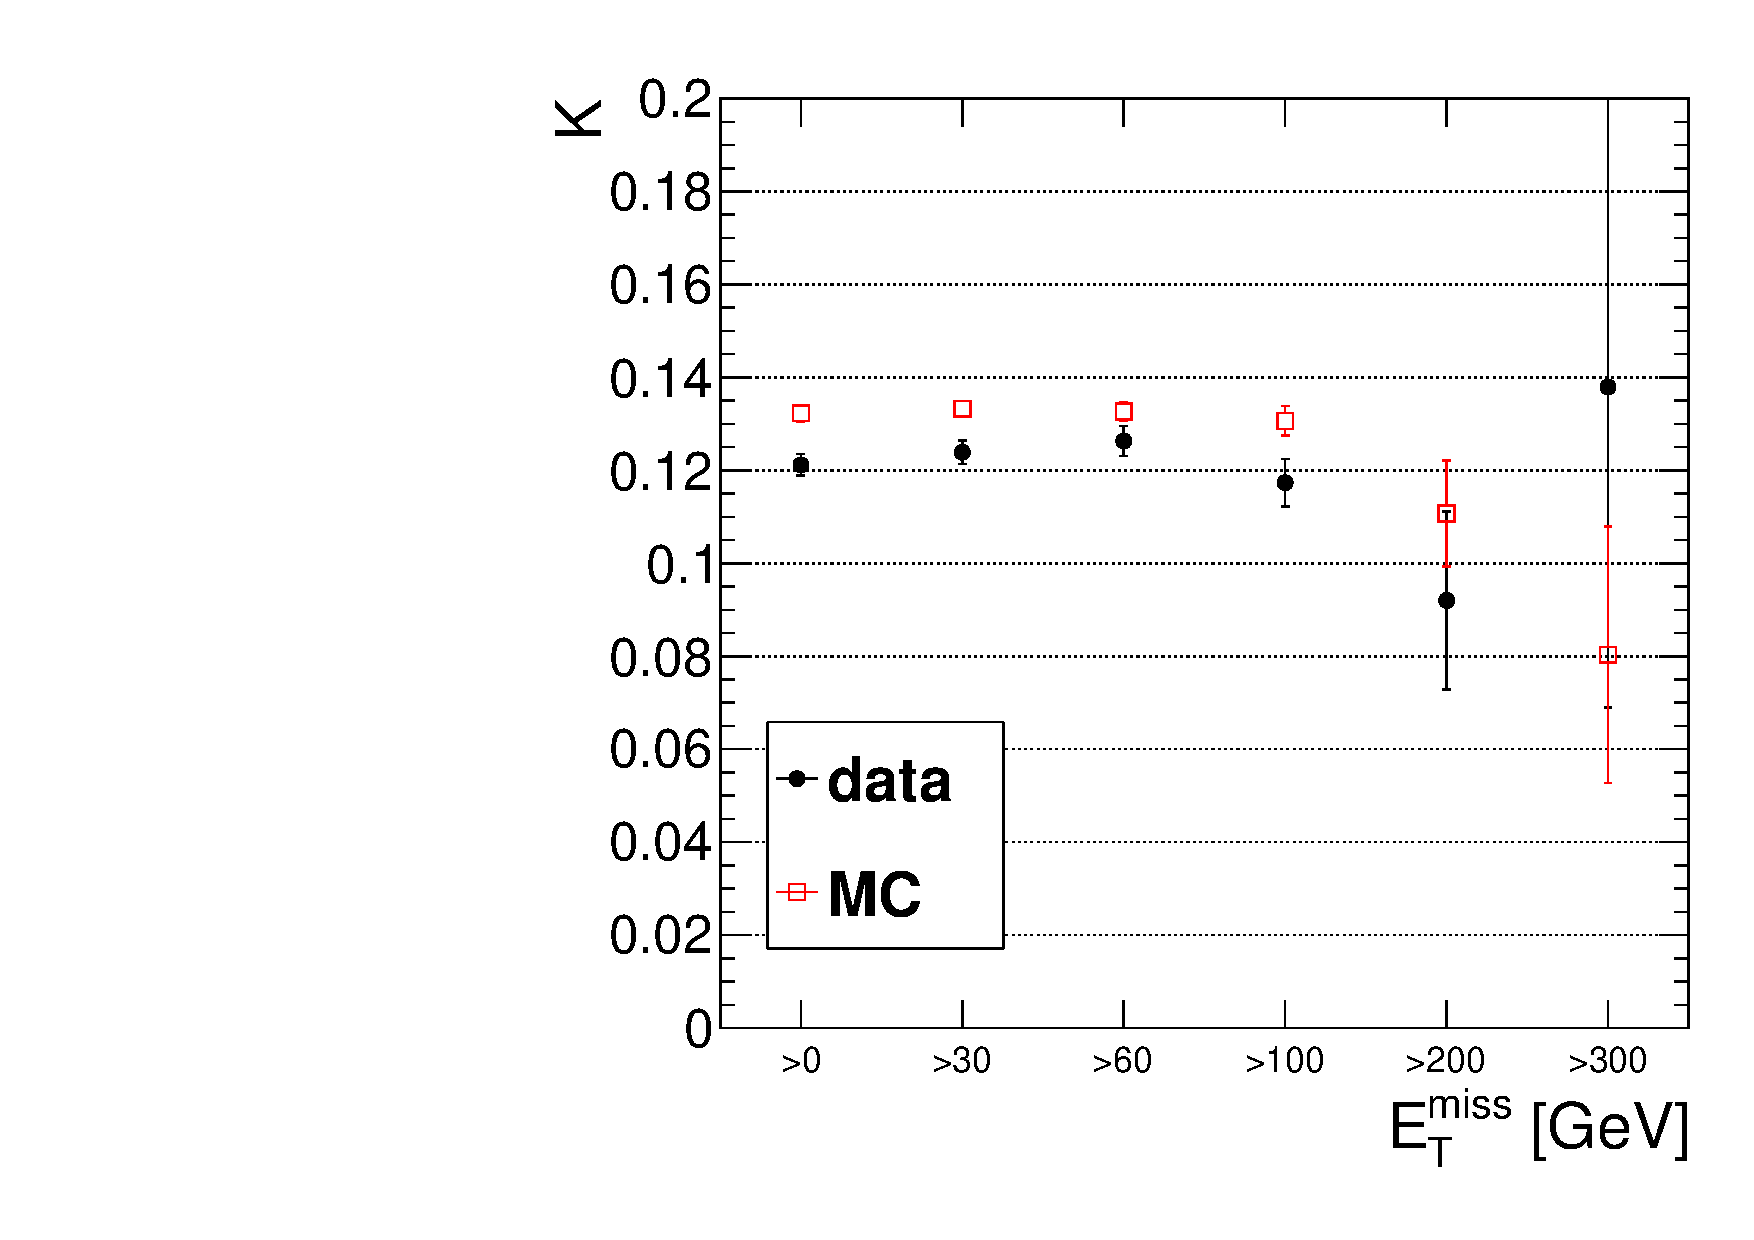
\includegraphics[width=0.4\textwidth]{plots/extractK_inclusive_pt2010_92fb.pdf} &
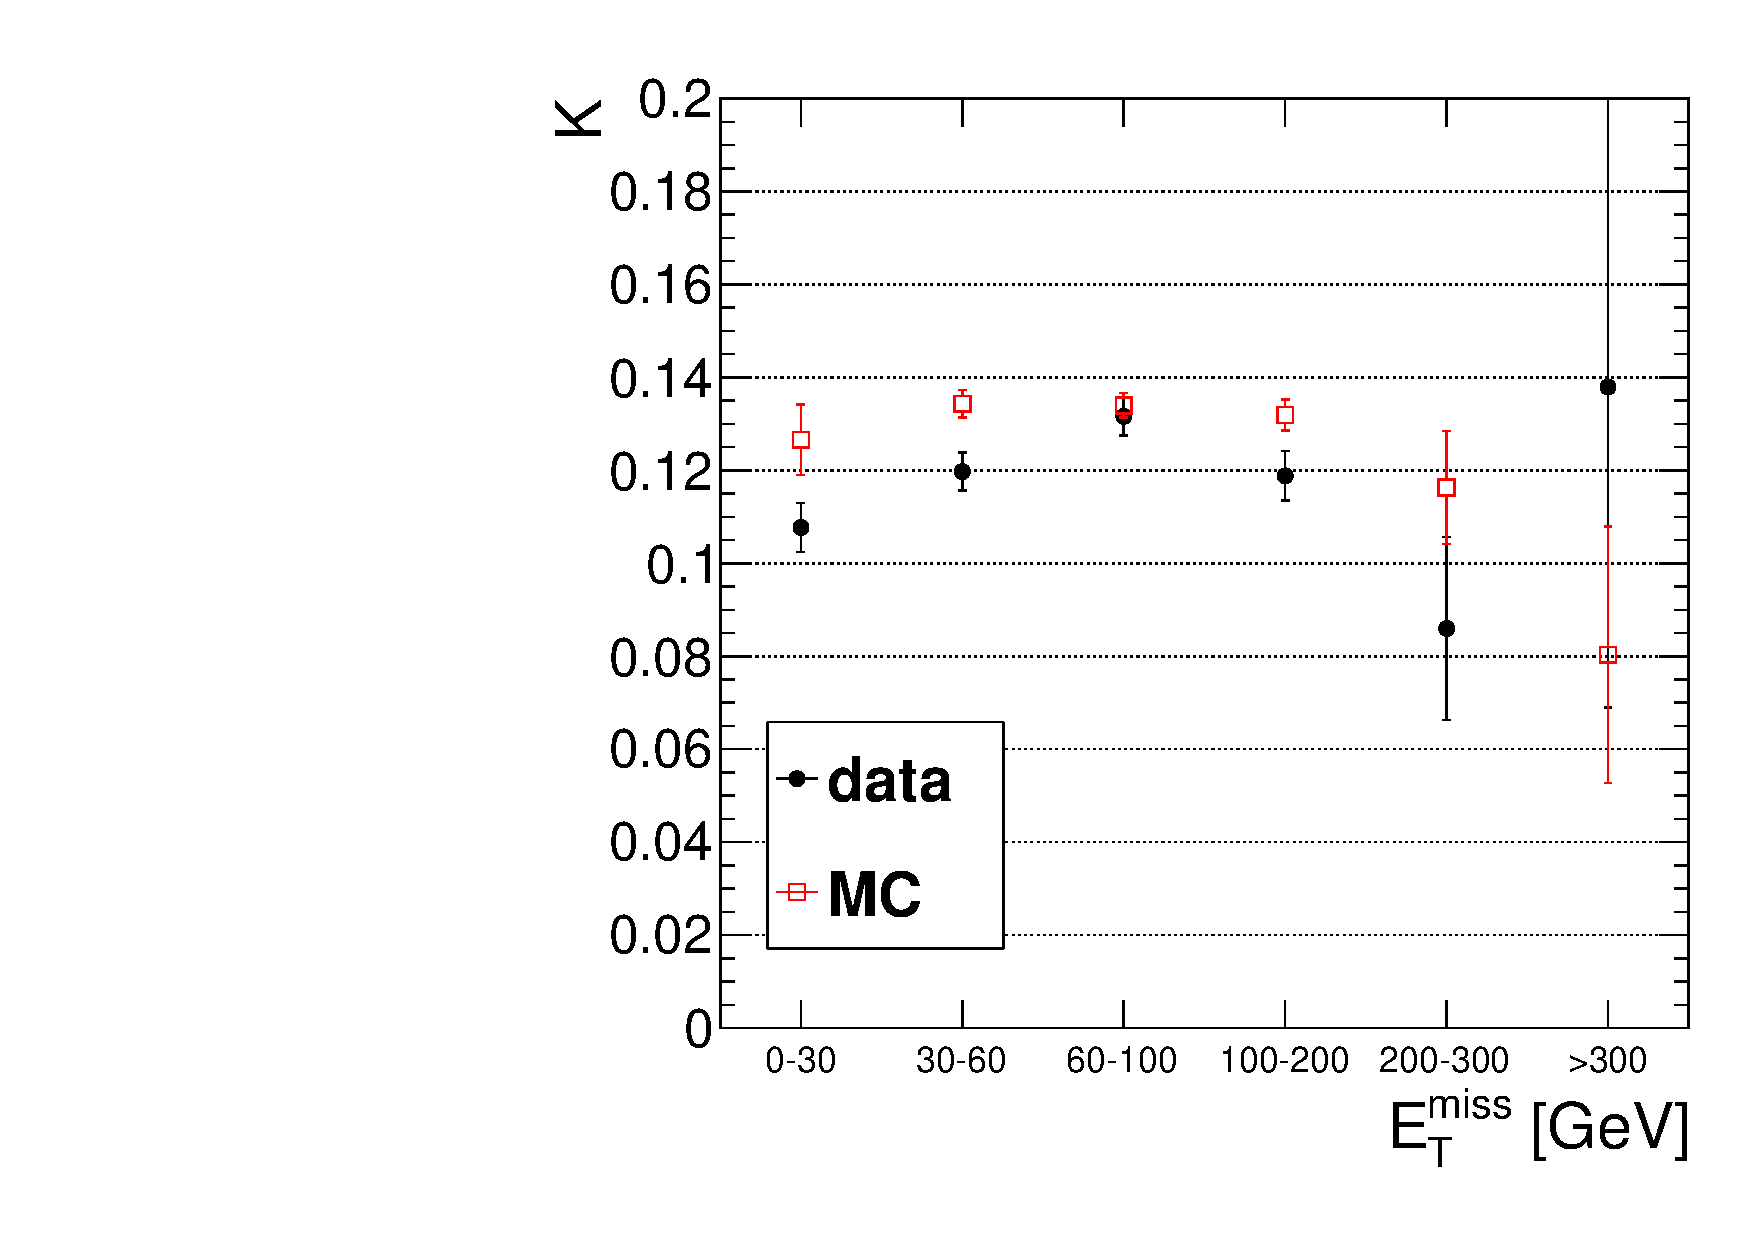
\includegraphics[width=0.4\textwidth]{plots/extractK_exclusive_pt2010_92fb.pdf} \\
\end{tabular}
\caption{\label{fig:K_incl_highmet}
The efficiency for e$\mu$ events to satisfy the dilepton mass requirement, $K$, in data and simulation for inclusive \MET\ intervals 
(left) and exclusive \MET\ intervals (right) for the dilepton \pt\ $>$ (20,10) GeV selection with at least 2 \pt\ $>$ 40 GeV jets
(used for the high \MET\ signal region). 
}
\end{center}
\end{figure}

\begin{comment}

Using selection : ((((leptype==2)&&(csc==0 && hbhe==1 && hcallaser==1 && ecaltp==1 && trkfail==1 && eebadsc==1 && hbhenew==1))&&(isdata==0 || (run<197556 || run>198913)))&&(njets40>=2))&&(lep1.pt()>20 && lep2.pt()>10)
Using weight    : vtxweight * weight
OF entries (total)  23031
OF entries (Z mass) 2791
K                   0.121184
Warning in <TROOT::Append>: Replacing existing TH1: htot (Potential memory leak).
Warning in <TROOT::Append>: Replacing existing TH1: hZ (Potential memory leak).

--------------------------------------------------------------
pfmet>0   && pfmet<30

data  : 
total : 3835
Z     : 413
K     : 0.11 +/- 0.005

MC    : 
total : 378.922
Z     : 47.9593
K     : 0.13 +/- 0.008
--------------------------------------------------------------


--------------------------------------------------------------
pfmet>30  && pfmet<60

data  : 
total : 7090
Z     : 849
K     : 0.12 +/- 0.004

MC    : 
total : 775.198
Z     : 104.129
K     : 0.13 +/- 0.003
--------------------------------------------------------------


--------------------------------------------------------------
pfmet>60  && pfmet<100

data  : 
total : 7598
Z     : 1000
K     : 0.13 +/- 0.004

MC    : 
total : 886.062
Z     : 118.721
K     : 0.13 +/- 0.003
--------------------------------------------------------------


--------------------------------------------------------------
pfmet>100 && pfmet<200

data  : 
total : 4258
Z     : 506
K     : 0.12 +/- 0.005

MC    : 
total : 538.442
Z     : 71.0424
K     : 0.13 +/- 0.003
--------------------------------------------------------------


--------------------------------------------------------------
pfmet>200 && pfmet<300

data  : 
total : 221
Z     : 19
K     : 0.09 +/- 0.020

MC    : 
total : 29.8247
Z     : 3.46834
K     : 0.12 +/- 0.012
--------------------------------------------------------------


--------------------------------------------------------------
pfmet>300

data  : 
total : 29
Z     : 4
K     : 0.14 +/- 0.069

MC    : 
total : 5.45734
Z     : 0.438259
K     : 0.08 +/- 0.028
--------------------------------------------------------------

root [1] extractK(false,false,false)
Using selection : ((((leptype==2)&&(csc==0 && hbhe==1 && hcallaser==1 && ecaltp==1 && trkfail==1 && eebadsc==1 && hbhenew==1))&&(isdata==0 || (run<197556 || run>198913)))&&(njets40>=2))&&(lep1.pt()>20 && lep2.pt()>10)
Using weight    : vtxweight * weight
OF entries (total)  23031
OF entries (Z mass) 2791
K                   0.121184
Info in <TCanvas::MakeDefCanvas>:  created default TCanvas with name c1

--------------------------------------------------------------
pfmet>0

data  : 
total : 23031
Z     : 2791
K     : 0.12 +/- 0.002

MC    : 
total : 2613.71
Z     : 345.768
K     : 0.13 +/- 0.002
--------------------------------------------------------------


--------------------------------------------------------------
pfmet>30

data  : 
total : 19196
Z     : 2378
K     : 0.12 +/- 0.003

MC    : 
total : 2234.8
Z     : 297.807
K     : 0.13 +/- 0.002
--------------------------------------------------------------


--------------------------------------------------------------
pfmet>60

data  : 
total : 12106
Z     : 1529
K     : 0.13 +/- 0.003

MC    : 
total : 1459.78
Z     : 193.67
K     : 0.13 +/- 0.002
--------------------------------------------------------------


--------------------------------------------------------------
pfmet>100

data  : 
total : 4508
Z     : 529
K     : 0.12 +/- 0.005

MC    : 
total : 573.708
Z     : 74.9489
K     : 0.13 +/- 0.003
--------------------------------------------------------------


--------------------------------------------------------------
pfmet>200

data  : 
total : 250
Z     : 23
K     : 0.09 +/- 0.019

MC    : 
total : 35.2821
Z     : 3.90659
K     : 0.11 +/- 0.011
--------------------------------------------------------------


--------------------------------------------------------------
pfmet>300

data  : 
total : 29
Z     : 4
K     : 0.14 +/- 0.069

MC    : 
total : 5.45734
Z     : 0.438259
K     : 0.08 +/- 0.028
--------------------------------------------------------------

\end{comment}


\begin{figure}[!ht]
\begin{center}
\begin{tabular}{cc}
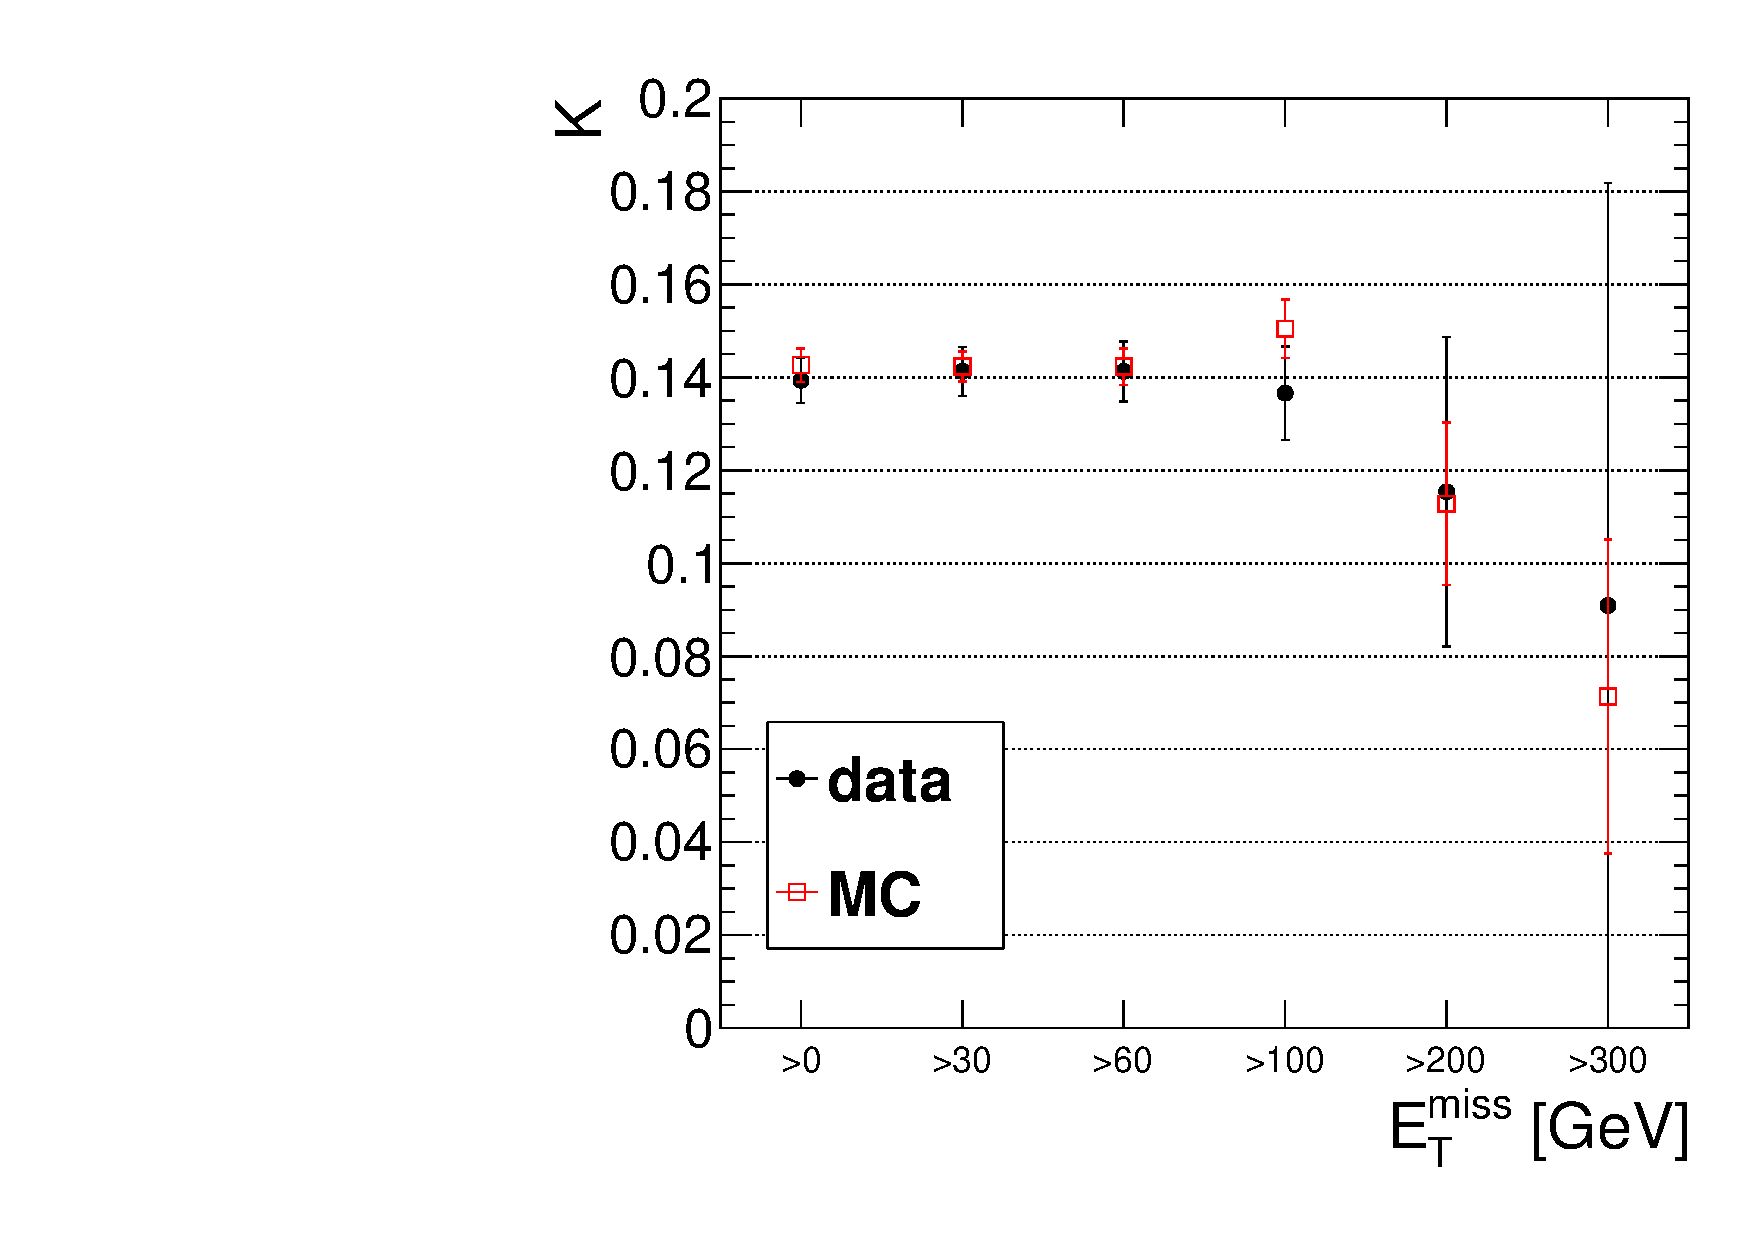
\includegraphics[width=0.4\textwidth]{plots/extractK_inclusive_lowmet.pdf} &
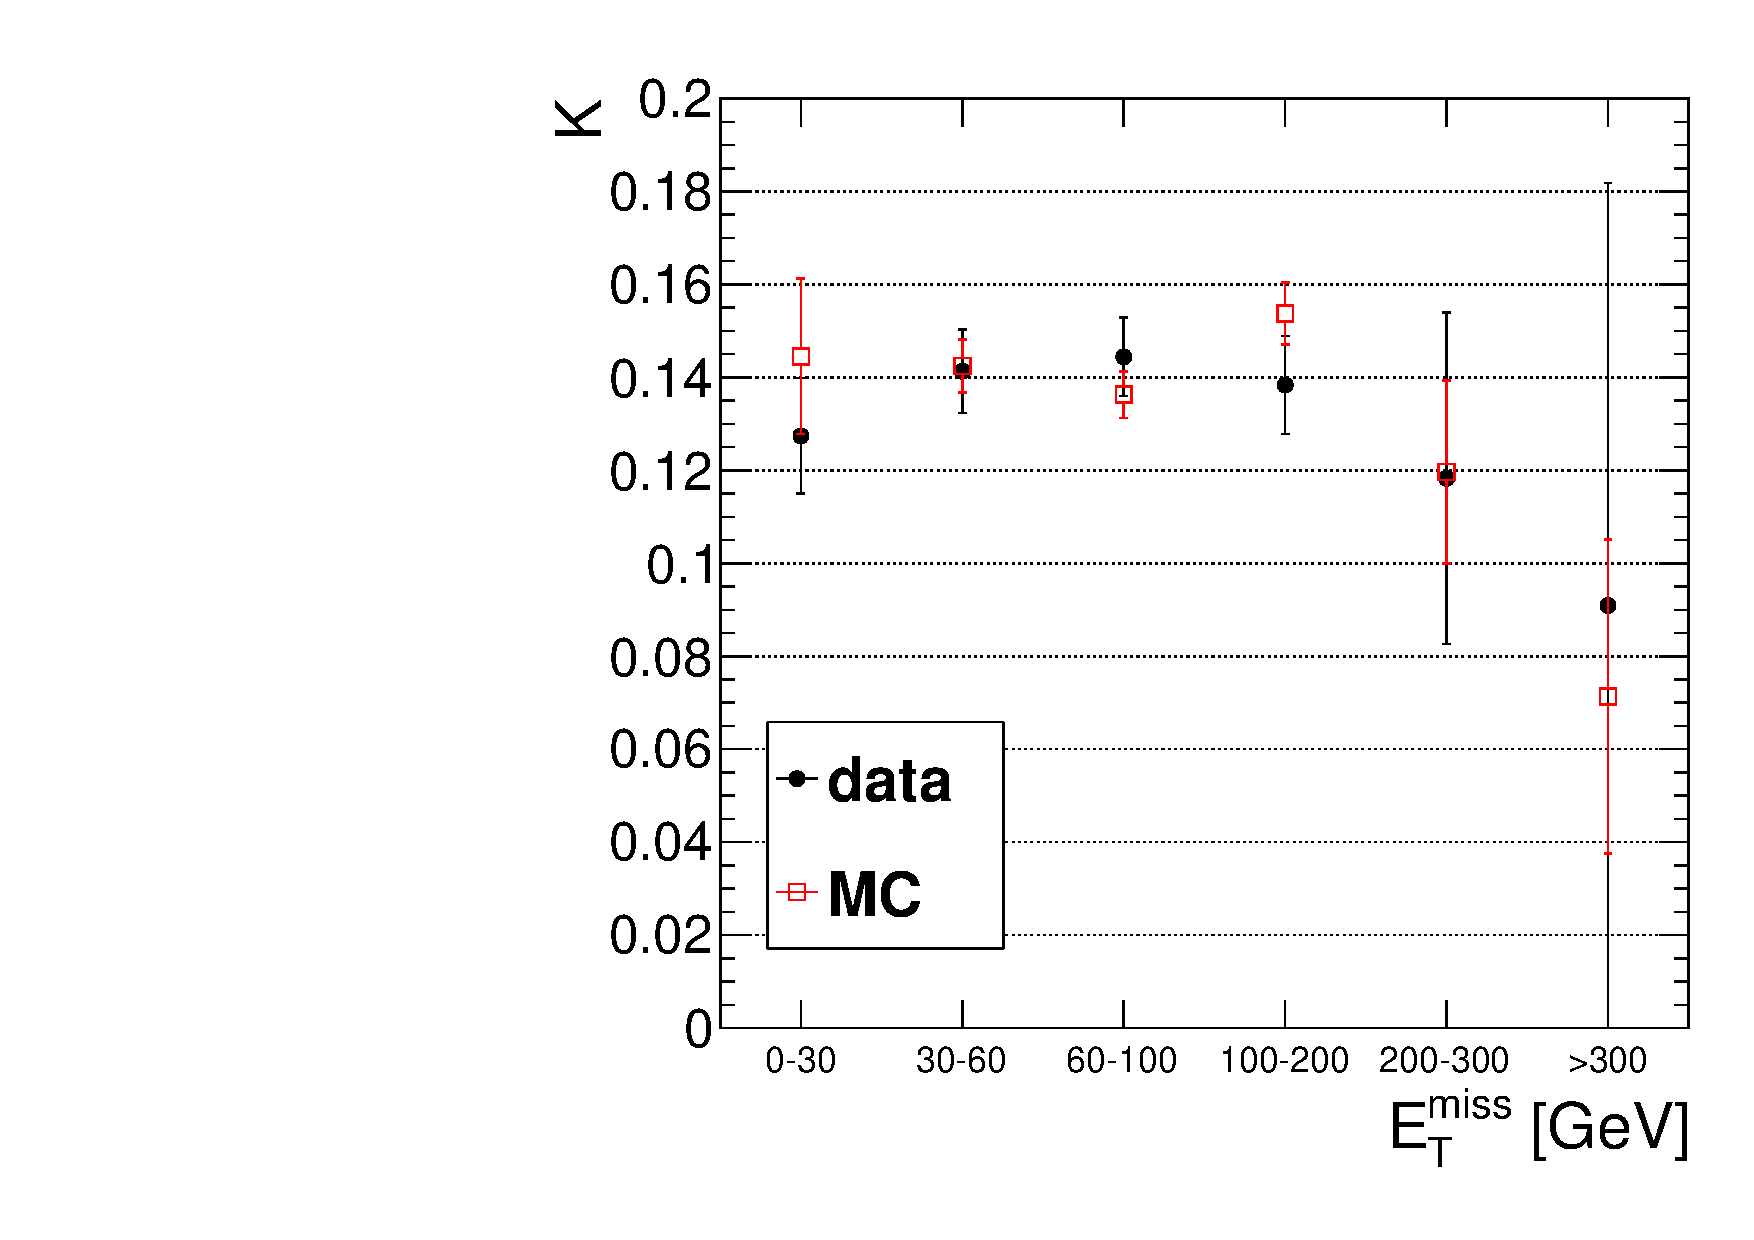
\includegraphics[width=0.4\textwidth]{plots/extractK_exclusive_lowmet.pdf} \\
\end{tabular}
\caption{\label{fig:K_incl_lowmet}
The efficiency for e$\mu$ events to satisfy the dilepton mass requirement, $K$, in data and simulation for inclusive \MET\ intervals 
(left) and exclusive \MET\ intervals (right) for the dilepton \pt\ $>$ (20,20) GeV selection with at least 3 \pt\ $>$ 40 GeV jets
(used for the low \MET\ signal region). 
}
\end{center}
\end{figure}

\begin{comment}

Using selection : ((((leptype==2)&&(csc==0 && hbhe==1 && hcallaser==1 && ecaltp==1 && trkfail==1 && eebadsc==1 && hbhenew==1))&&(isdata==0 || (run<197556 || run>198913)))&&(njets40>=3))&&(lep1.pt()>20 && lep2.pt()>20)
Using weight    : vtxweight * weight
OF entries (total)  5934
OF entries (Z mass) 827
K                   0.139366

--------------------------------------------------------------
pfmet>0

data  : 
total : 5934
Z     : 827
K     : 0.14 +/- 0.005

MC    : 
total : 725.106
Z     : 103.443
K     : 0.14 +/- 0.004
--------------------------------------------------------------


--------------------------------------------------------------
pfmet>30

data  : 
total : 5110
Z     : 722
K     : 0.14 +/- 0.005

MC    : 
total : 625.723
Z     : 89.0789
K     : 0.14 +/- 0.003
--------------------------------------------------------------


--------------------------------------------------------------
pfmet>60

data  : 
total : 3362
Z     : 475
K     : 0.14 +/- 0.006

MC    : 
total : 418.375
Z     : 59.5404
K     : 0.14 +/- 0.004
--------------------------------------------------------------


--------------------------------------------------------------
pfmet>100

data  : 
total : 1347
Z     : 184
K     : 0.14 +/- 0.010

MC    : 
total : 177.754
Z     : 26.7455
K     : 0.15 +/- 0.006
--------------------------------------------------------------


--------------------------------------------------------------
pfmet>200

data  : 
total : 104
Z     : 12
K     : 0.12 +/- 0.033

MC    : 
total : 14.1212
Z     : 1.59283
K     : 0.11 +/- 0.018
--------------------------------------------------------------


--------------------------------------------------------------
pfmet>300

data  : 
total : 11
Z     : 1
K     : 0.09 +/- 0.091

MC    : 
total : 2.00086
Z     : 0.142752
K     : 0.07 +/- 0.034
--------------------------------------------------------------

root [3] Info in <TCanvas::Print>: pdf file /home/users/benhoob/ZMet2012/plots/extractK_inclusive_lowmet.pdf has been created

root [3] 
root [3] extractK(true,false,false)
Using selection : ((((leptype==2)&&(csc==0 && hbhe==1 && hcallaser==1 && ecaltp==1 && trkfail==1 && eebadsc==1 && hbhenew==1))&&(isdata==0 || (run<197556 || run>198913)))&&(njets40>=3))&&(lep1.pt()>20 && lep2.pt()>20)
Using weight    : vtxweight * weight
OF entries (total)  5934
OF entries (Z mass) 827
K                   0.139366
Warning in <TFile::Append>: Replacing existing TH1: htot (Potential memory leak).
Warning in <TFile::Append>: Replacing existing TH1: hZ (Potential memory leak).

--------------------------------------------------------------
pfmet>0   && pfmet<30

data  : 
total : 824
Z     : 105
K     : 0.13 +/- 0.012

MC    : 
total : 99.3853
Z     : 14.3649
K     : 0.14 +/- 0.017
--------------------------------------------------------------


--------------------------------------------------------------
pfmet>30  && pfmet<60

data  : 
total : 1748
Z     : 247
K     : 0.14 +/- 0.009

MC    : 
total : 207.368
Z     : 29.5391
K     : 0.14 +/- 0.006
--------------------------------------------------------------


--------------------------------------------------------------
pfmet>60  && pfmet<100

data  : 
total : 2015
Z     : 291
K     : 0.14 +/- 0.008

MC    : 
total : 240.615
Z     : 32.7949
K     : 0.14 +/- 0.005
--------------------------------------------------------------


--------------------------------------------------------------
pfmet>100 && pfmet<200

data  : 
total : 1243
Z     : 172
K     : 0.14 +/- 0.011

MC    : 
total : 163.632
Z     : 25.1526
K     : 0.15 +/- 0.007
--------------------------------------------------------------


--------------------------------------------------------------
pfmet>200 && pfmet<300

data  : 
total : 93
Z     : 11
K     : 0.12 +/- 0.036

MC    : 
total : 12.1203
Z     : 1.45008
K     : 0.12 +/- 0.020
--------------------------------------------------------------


--------------------------------------------------------------
pfmet>300

data  : 
total : 11
Z     : 1
K     : 0.09 +/- 0.091

MC    : 
total : 2.00086
Z     : 0.142752
K     : 0.07 +/- 0.034
--------------------------------------------------------------


\end{comment}

The strategy is to select Z$\to\ell\ell$ candidates ($81<m_{\ell\ell}<101$ GeV) with jet requirements corresponding to the
low-\MET\ and high-\MET\ signal regions, and compare the observed \MET\ distribution to the sum of the predictions from the 
\zjets\ background (from the \MET\ templates method based on the \gjets\ data control sample), the flavor-symmetric background predicted
from e$\mu$ data events, and MC contributions from WZ/ZZ, as well as the rare SM processes with Z bosons ($t\bar{t}\rm{Z}$ and ZZZ, ZZW, ZWW).

The results of the low \MET\ signal region are displayed in Fig.~\ref{fig:results_lowmet} and summarized in Table~\ref{tab:results_lowmet},
separately for the Run2012A+B data (5.1 fb$^{-1}$) and Run2012C data (4.1 fb$^{-1}$).
In the Run2012A+B data, we observed a 1.6$\sigma$ excess for \MET\ $>$ 100 GeV, corresponding to the low \MET\ signal region.
However, this excess does not persist in Run2012C data, where we observe good agreement between the data and the predicted background.
In the combined Run2012A+B+C data (Fig.~\ref{fig:results_fulledge} and Table~\ref{tab:results_edgefull}) we observe reasonable
agreement over the full \MET\ range. In the \MET\ $>$ 100 GeV region we observe 288 events with a predicted background of $251\pm33$,
representing an excess of 1.0$\sigma$.

The results of the high \MET\ signal region are displayed in Fig.~\ref{fig:results_highmet} and summarized in Table~\ref{tab:results_highmet},
separately for the Run2012A+B data (5.1 fb$^{-1}$) and Run2012C data (4.1 fb$^{-1}$).
In both periods we observe good agreement between the data and predicted background over the full \MET\ range.
In the \MET\ $>$ 150 GeV region corresponding to the high \MET\ signal region in the full sample, we observe 167 events with a predicted
background of $177\pm25$ events, representing a deficit of -0.4$\sigma$.

\clearpage

\begin{figure}[!h]
\begin{center}
\begin{tabular}{cc}
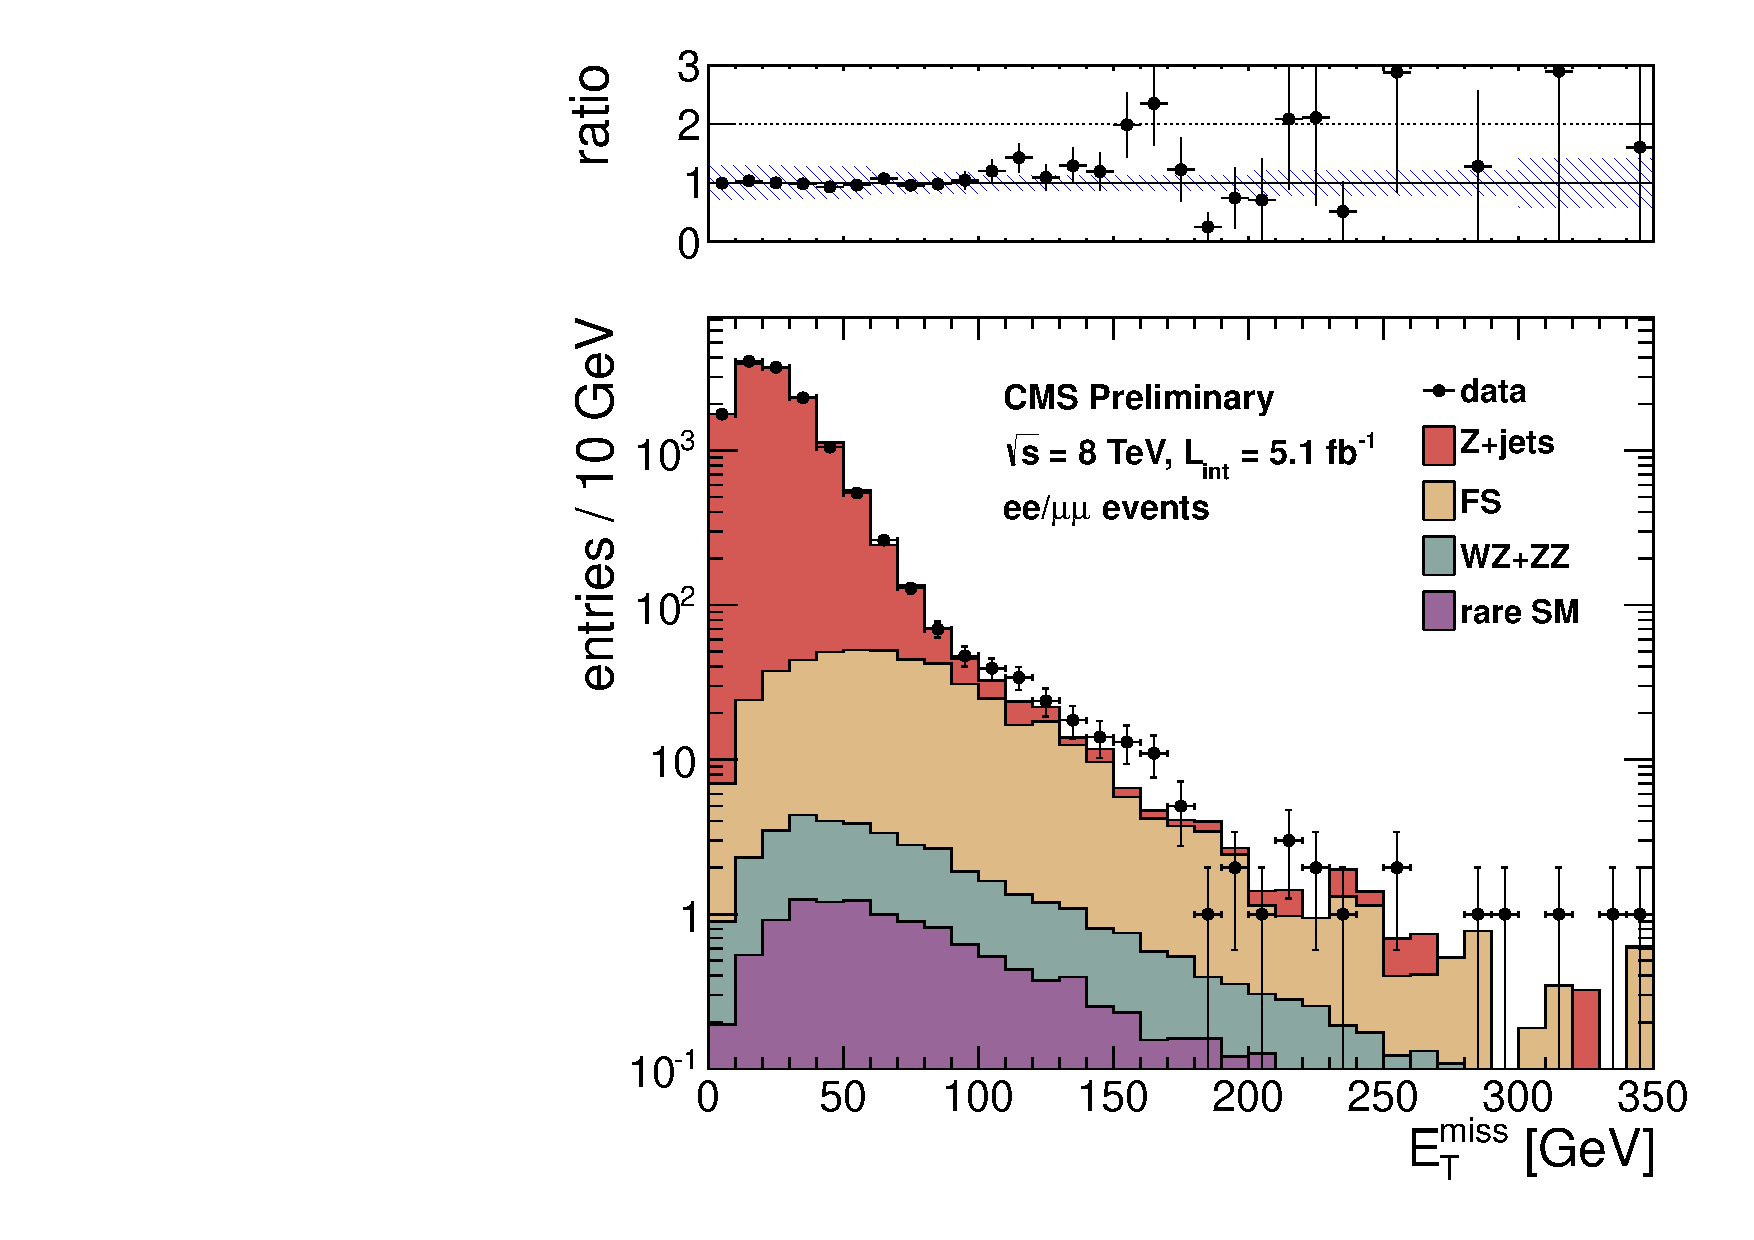
\includegraphics[width=0.45\textwidth]{plots/pfmet_pt40_2012AB_lowMet_all.pdf}
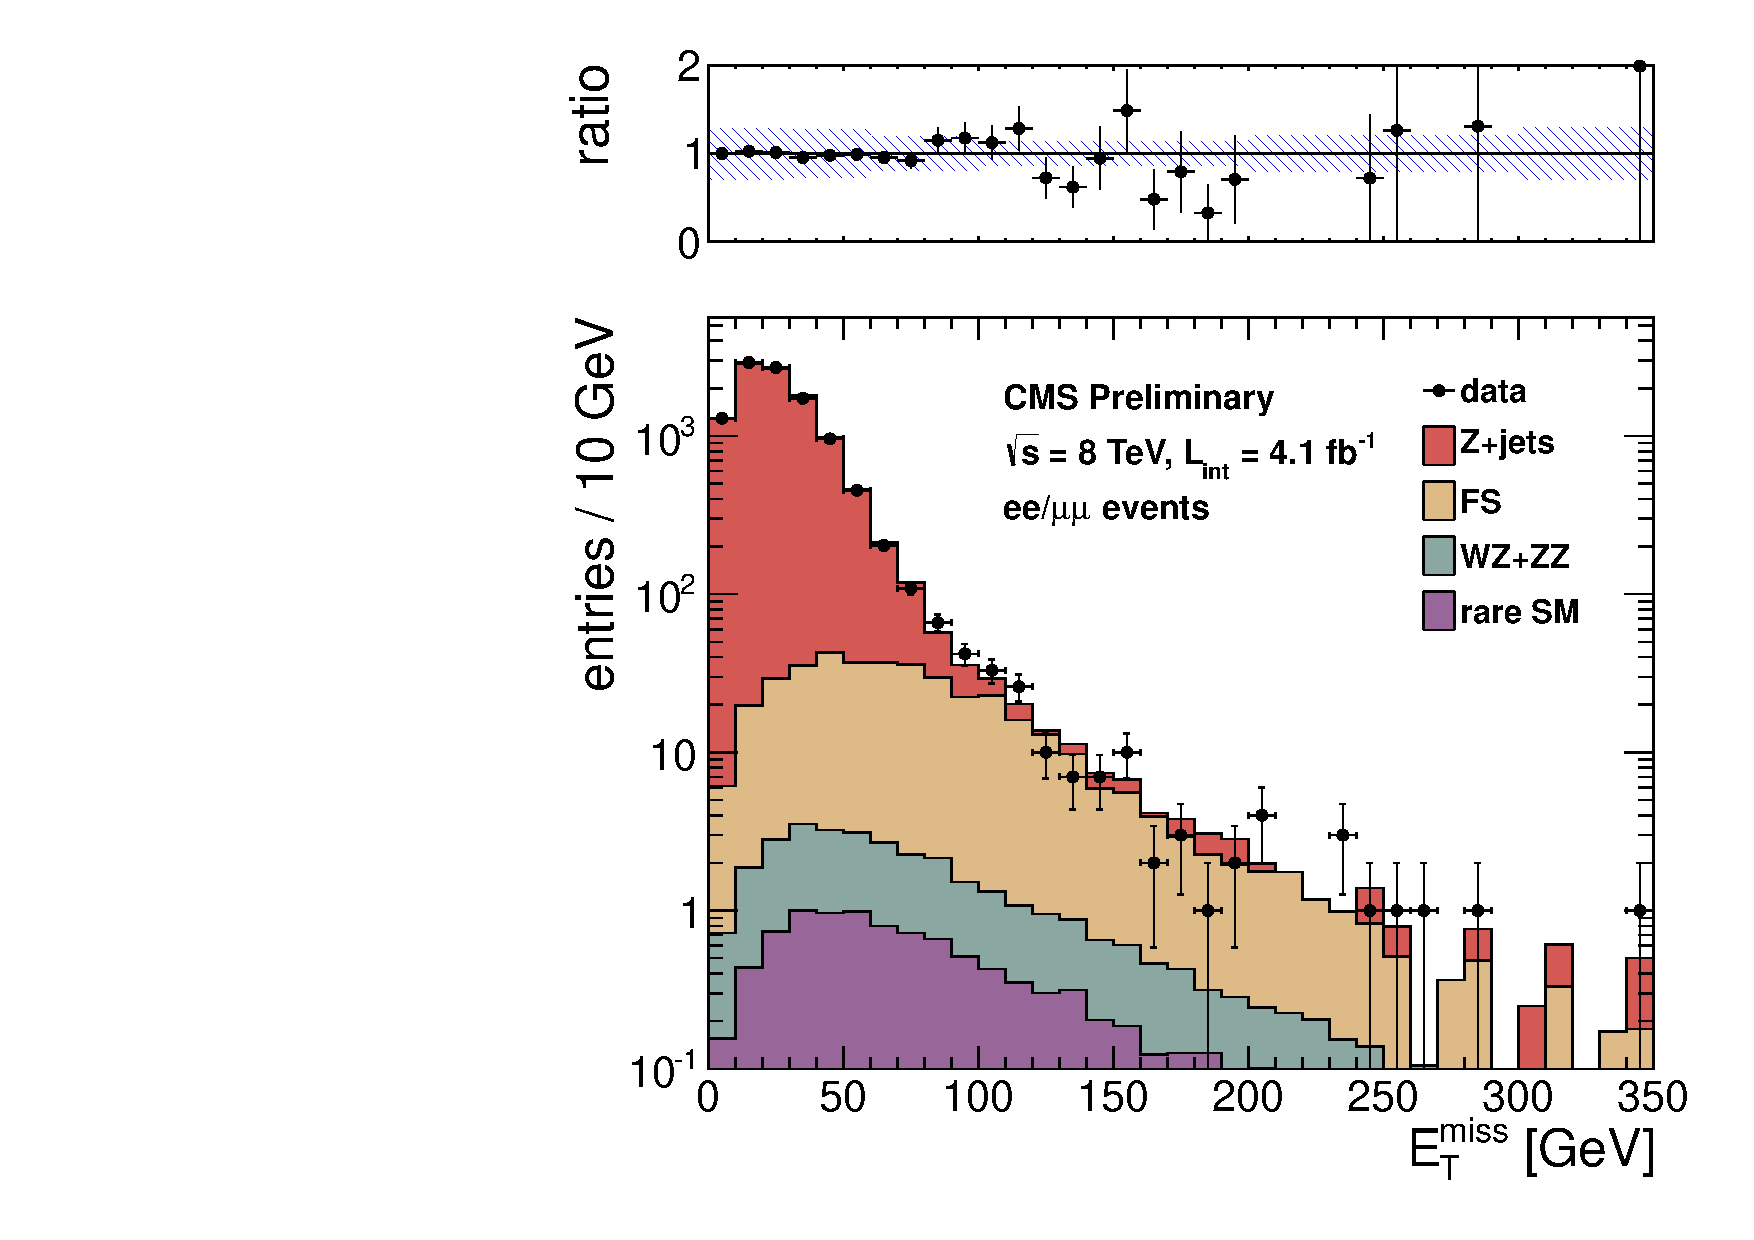
\includegraphics[width=0.45\textwidth]{plots/pfmet_pt40_2012C_lowMet_all.pdf}
%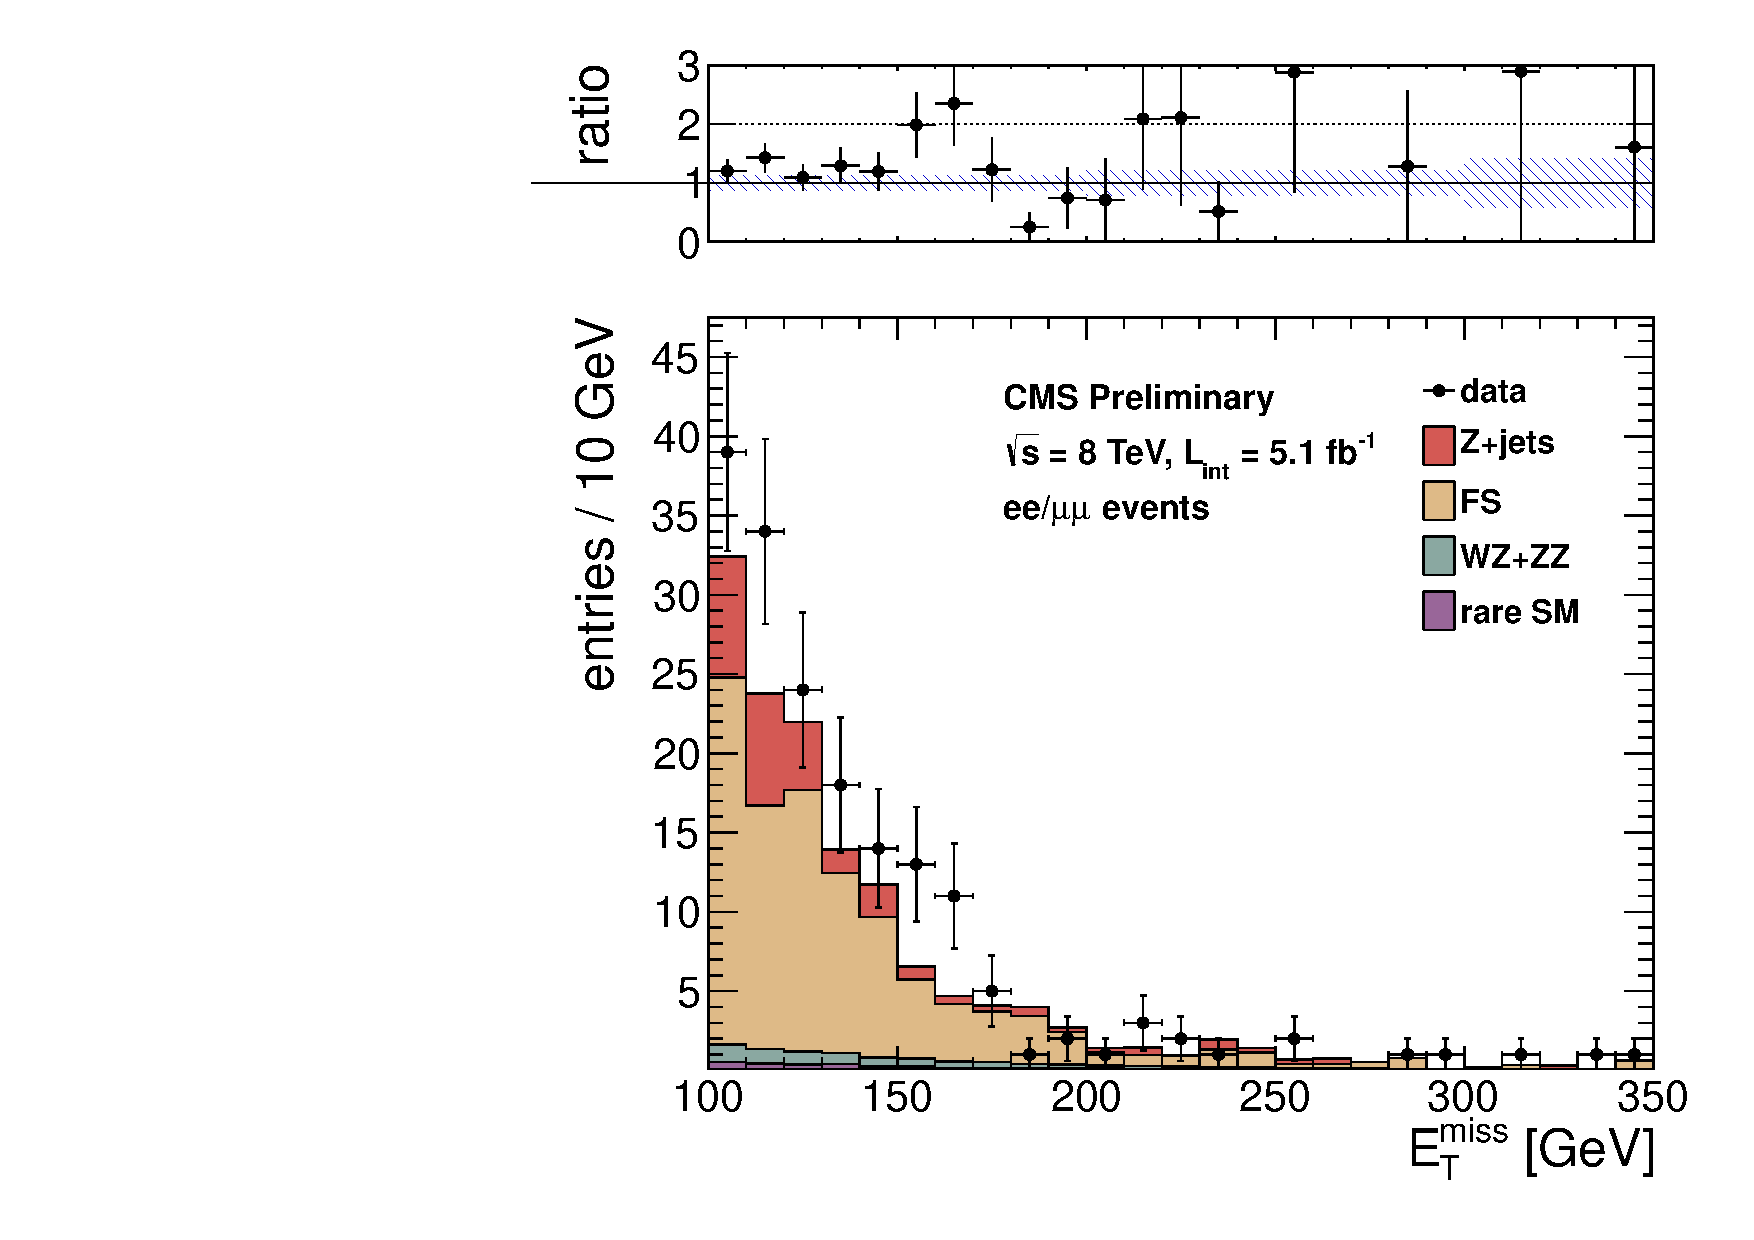
\includegraphics[width=0.48\textwidth]{plots/pfmet_pt40_2012AB_lowMet_all_linear.pdf}
\end{tabular}
\caption{\footnotesize Results for the low \MET\ signal region. 
The results for 5.1 fb$^{-1}$ 2012A+B data are displayed on the left, the results for 4.1 fb$^{-1}$ 2012C data are displayed on the right. 
%The left plot shows the full \MET\ range, the right plot is zoomed in on the \MET\ $>$ 100 GeV region.
The observed \MET\ distribution (black points) is compared with the sum of the predicted \MET\
distributions from \zjets, flavor-symmetric backgrounds, WZ+ZZ backgrounds, and rare SM backgrounds. 
The ratio of observed to predicted yields in each bin is
indicated. The error bars indicate the statistical uncertainty in the data and the shaded band indicates the total background uncertainty.
\label{fig:results_lowmet}
}
\end{center}
\end{figure}

\begin{table}[htb]
\begin{center}
\footnotesize
\caption{\label{tab:results_lowmet} \footnotesize Results for the low \MET\ signal region. 
The results for 5.1 fb$^{-1}$ 2012A+B data are displayed in the top table, the results for 4.1 fb$^{-1}$ 2012C data are displayed in the bottom table. 
The total background is the sum of the \zjets\ background predicted from
the \MET\ templates method (\zjets\ bkg), the flavor-symmetric background predicted from e$\mu$ events (FS bkg), the WZ and ZZ backgrounds predicted from MC
(WZ bkg and ZZ bkg) and the rare SM backgrounds. All uncertainties include both the statistical and systematic components. The Gaussian significance of the deviation between the data 
and total background is indicated for signal regions with at least 20 observed events. }
\begin{tabular}{l|c|c|c|c|c|c}

\hline
\hline

\begin{comment}
Using pfmet out-of-the-box
Using pT > 40 GeV jets, low MET signal region
WZ/ZZ selection : ((((((leptype==0 && (ee==1 || isdata==0))||(leptype==1 && (mm==1 || isdata==0)))&&(ngennu>0))&&(csc==0 && hbhe==1 && hcallaser==1 && ecaltp==1 && trkfail==1 && eebadsc==1 && hbhenew==1))&&(dilmass>81 && dilmass<101))&&(lep1.pt()>20.0 && lep2.pt()>20.0))&&(njets40>=3)
WZ/ZZ weight    : weight * 5.1 * vtxweight * trgeff
Opening ../output/V00-01-04/babylooper_data_ALL_53X_PhotonStitchedTemplate_pfmet_pt40_2012AB_lowMet.root
B-veto?   0
K         0.14
ee+mm channels: scale em yield by 0.99
Yields in 0-60 GeV region
data   : 12728
gjets  : 13041.3
OF     : 194.733
WZ     : 12.3421
ZZ     : 1.31265
Rare   : 5.32478
Scaling gjets by : 0.959591
SF events 13412
OF events 3254

ee/#mu#mu events
\end{comment}


                      &   \MET\ $>$ 0 GeV   &  \MET\ $>$ 30 GeV   &  \MET\ $>$ 60 GeV   & \MET\ $>$ 100 GeV   & \MET\ $>$ 200 GeV   & \MET\ $>$ 300 GeV  \\
\hline
        \zjets\ bkg   &  12870 $\pm$ 3862   &   4118 $\pm$ 1236   &     356 $\pm$ 107   &    27.5 $\pm$ 8.5   &     2.6 $\pm$ 1.1   &     0.3 $\pm$ 0.3  \\
             FS bkg   &      451 $\pm$ 70   &      389 $\pm$ 61   &      256 $\pm$ 40   &   99.1 $\pm$ 15.8   &     6.9 $\pm$ 1.8   &     1.0 $\pm$ 0.6  \\
             WZ bkg   &   24.1 $\pm$ 16.9   &   19.5 $\pm$ 13.7   &    11.8 $\pm$ 8.3   &     5.6 $\pm$ 3.9   &     1.1 $\pm$ 1.0   &     0.2 $\pm$ 0.2  \\
             ZZ bkg   &     4.3 $\pm$ 2.2   &     3.9 $\pm$ 2.0   &     3.0 $\pm$ 1.5   &     1.9 $\pm$ 1.0   &     0.5 $\pm$ 0.4   &     0.1 $\pm$ 0.1  \\
        rare SM bkg   &    12.2 $\pm$ 6.1   &    10.5 $\pm$ 5.3   &     6.9 $\pm$ 3.5   &     3.5 $\pm$ 1.8   &     0.7 $\pm$ 0.6   &     0.2 $\pm$ 0.2  \\
\hline
          total bkg   &  13362 $\pm$ 3862   &   4541 $\pm$ 1238   &     634 $\pm$ 115   & {\bf  138 $\pm$ 18} &    11.8 $\pm$ 2.5   &     1.8 $\pm$ 0.8  \\
               data   &             13412   &              4461   &               684   &     {\bf     175 }  &                14   &                 3  \\
       significance   &       0.0$\sigma$   &      -0.1$\sigma$   &       0.4$\sigma$   & {\bf 1.6$\sigma$ }  &       0.5$\sigma$   &                    \\

\hline
\hline


\begin{comment}
Using pfmet out-of-the-box
Using pT > 40 GeV jets, low MET signal region
WZ/ZZ selection : ((((((leptype==0 && (ee==1 || isdata==0))||(leptype==1 && (mm==1 || isdata==0)))&&(ngennu>0))&&(csc==0 && hbhe==1 && hcallaser==1 && ecaltp==1 && trkfail==1 && eebadsc==1 && hbhenew==1))&&(dilmass>81 && dilmass<101))&&(lep1.pt()>20.0 && lep2.pt()>20.0))&&(njets40>=3)
WZ/ZZ weight    : weight * 4.1 * vtxweight * trgeff
Opening ../output/V00-01-04/babylooper_data_ALL_53X_PhotonStitchedTemplate_pfmet_pt40_2012C_lowMet.root
B-veto?   0
K         0.14
ee+mm channels: scale em yield by 0.99
Yields in 0-60 GeV region
data   : 10054
gjets  : 10255.2
OF     : 155.509
WZ     : 9.92205
ZZ     : 1.05527
Rare   : 4.2807
Scaling gjets by : 0.963729
SF events 10587
OF events 2572

ee/#mu#mu events
\end{comment}

                      &   \MET\ $>$ 0 GeV   &  \MET\ $>$ 30 GeV   &  \MET\ $>$ 60 GeV   & \MET\ $>$ 100 GeV   & \MET\ $>$ 200 GeV   & \MET\ $>$ 300 GeV  \\
\hline
        \zjets\ bkg   &  10203 $\pm$ 3061   &   3449 $\pm$ 1035   &      320 $\pm$ 97   &    20.5 $\pm$ 6.3   &     2.1 $\pm$ 0.6   &     0.8 $\pm$ 0.2  \\
             FS bkg   &      356 $\pm$ 56   &      307 $\pm$ 48   &      201 $\pm$ 32   &   84.5 $\pm$ 13.5   &     7.2 $\pm$ 1.9   &     0.6 $\pm$ 0.4  \\
             WZ bkg   &   19.4 $\pm$ 13.6   &   15.7 $\pm$ 11.0   &     9.5 $\pm$ 6.6   &     4.5 $\pm$ 3.2   &     0.9 $\pm$ 0.8   &     0.2 $\pm$ 0.2  \\
             ZZ bkg   &     3.5 $\pm$ 1.8   &     3.1 $\pm$ 1.6   &     2.4 $\pm$ 1.2   &     1.5 $\pm$ 0.8   &     0.4 $\pm$ 0.4   &     0.1 $\pm$ 0.1  \\
        rare SM bkg   &     9.8 $\pm$ 4.9   &     8.5 $\pm$ 4.3   &     5.5 $\pm$ 2.8   &     2.8 $\pm$ 1.5   &     0.6 $\pm$ 0.5   &     0.1 $\pm$ 0.1  \\
\hline
          total bkg   &  10592 $\pm$ 3062   &   3783 $\pm$ 1036   &     538 $\pm$ 102   &{\bf  114 $\pm$ 15}  &    11.2 $\pm$ 2.2   &     1.8 $\pm$ 0.5  \\
               data   &             10587   &              3673   &               533   &       {\bf   113 }  &                12   &                 1  \\
       significance   &      -0.0$\sigma$   &      -0.1$\sigma$   &      -0.0$\sigma$   & {\bf-0.0$\sigma$ }  &                     &                    \\
\hline
\hline



\end{tabular}
\end{center}
\end{table}

\clearpage


\begin{figure}[!h]
\begin{center}
\begin{tabular}{cc}
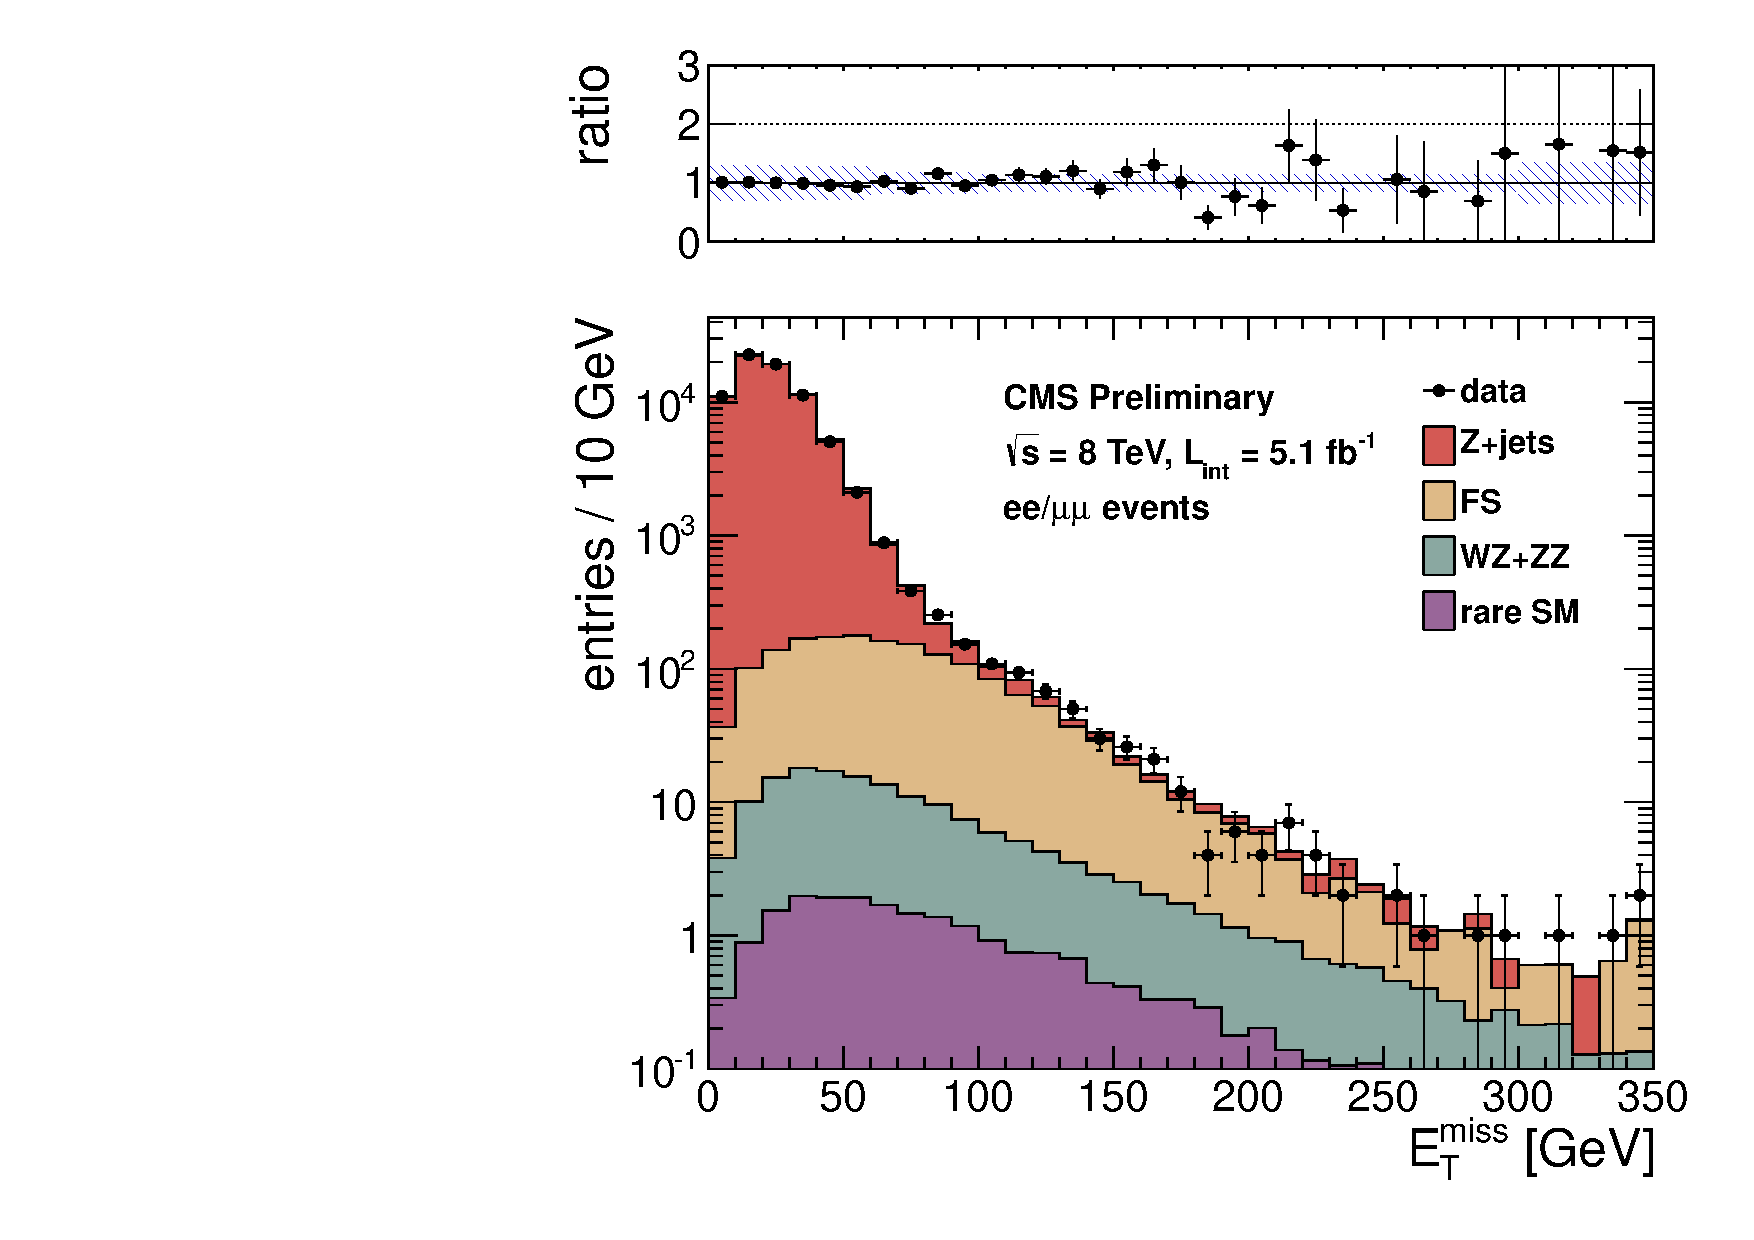
\includegraphics[width=0.45\textwidth]{plots/pfmet_pt40_2012AB_highMet_all.pdf}
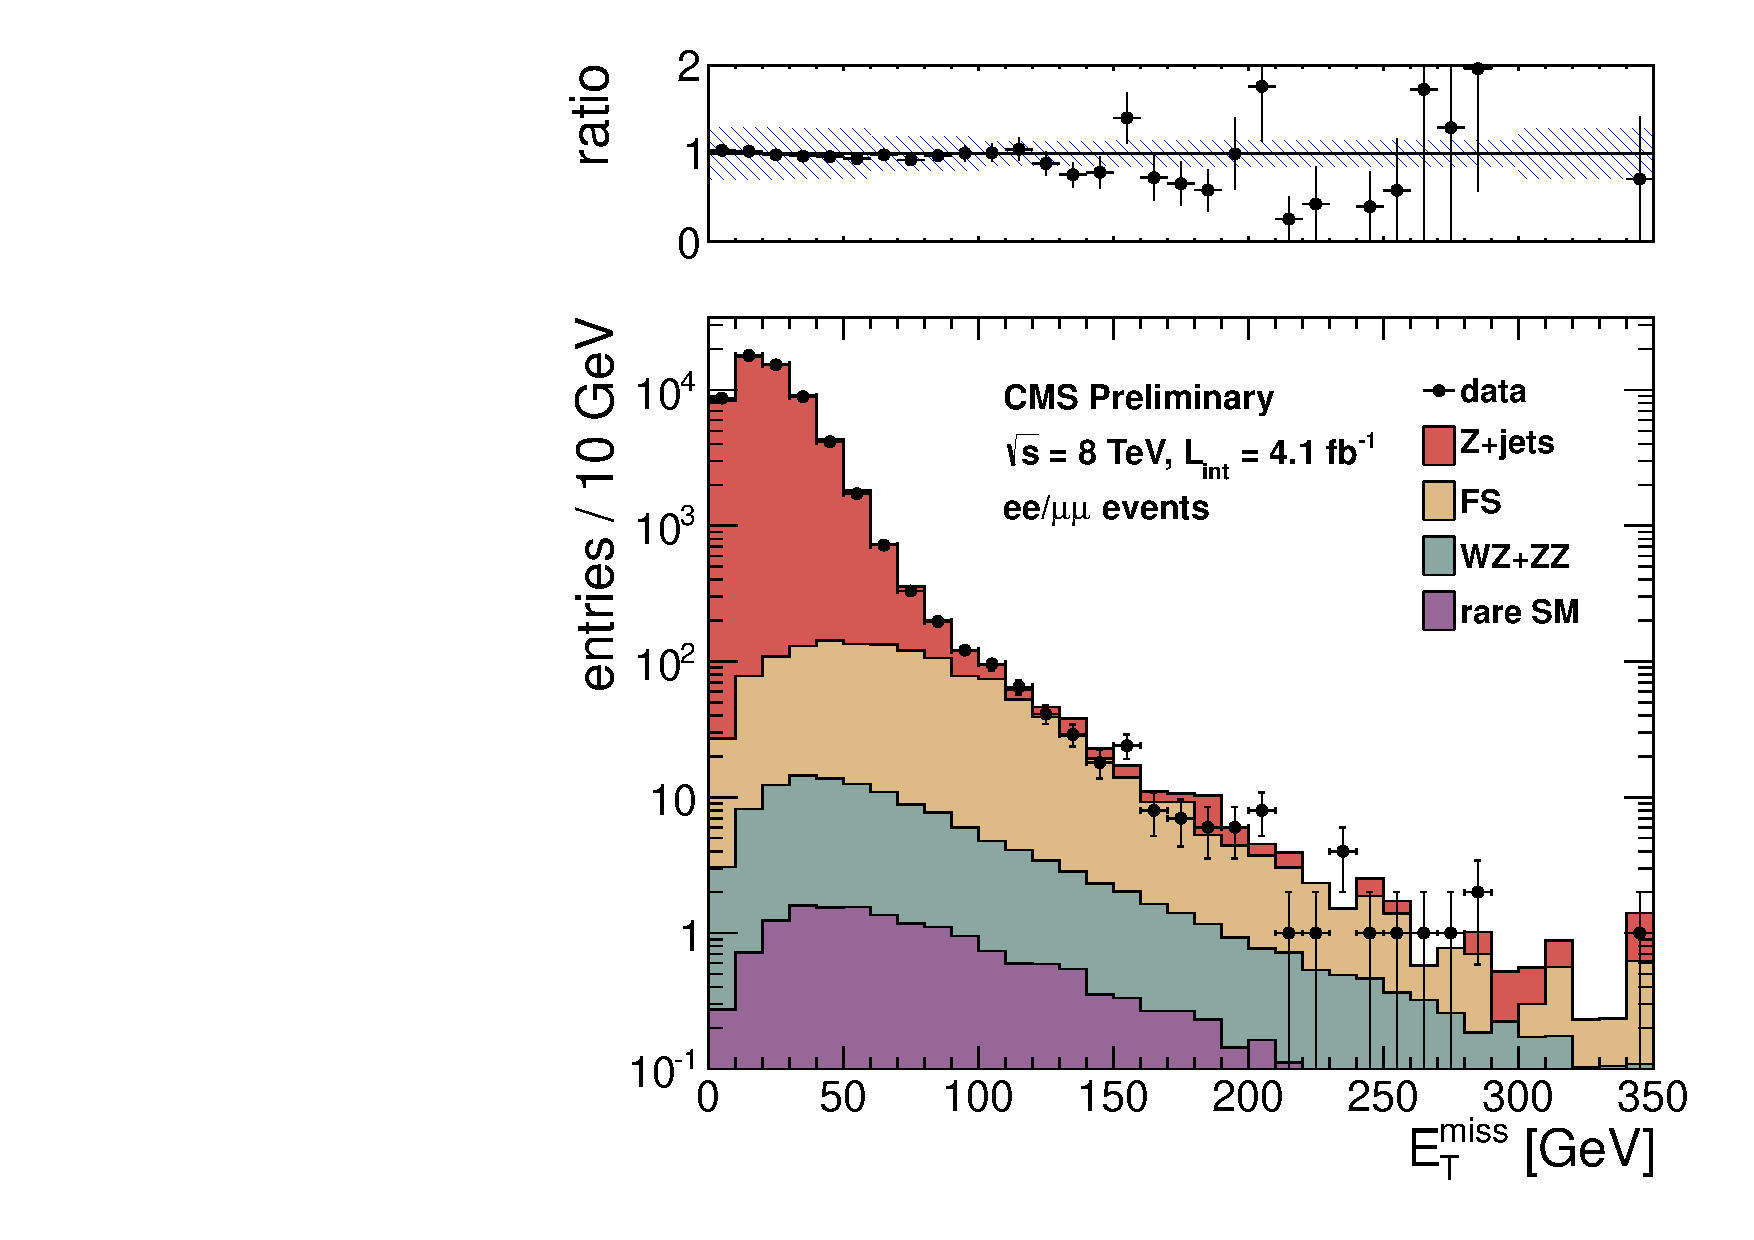
\includegraphics[width=0.45\textwidth]{plots/pfmet_pt40_2012C_highMet_all.pdf}
%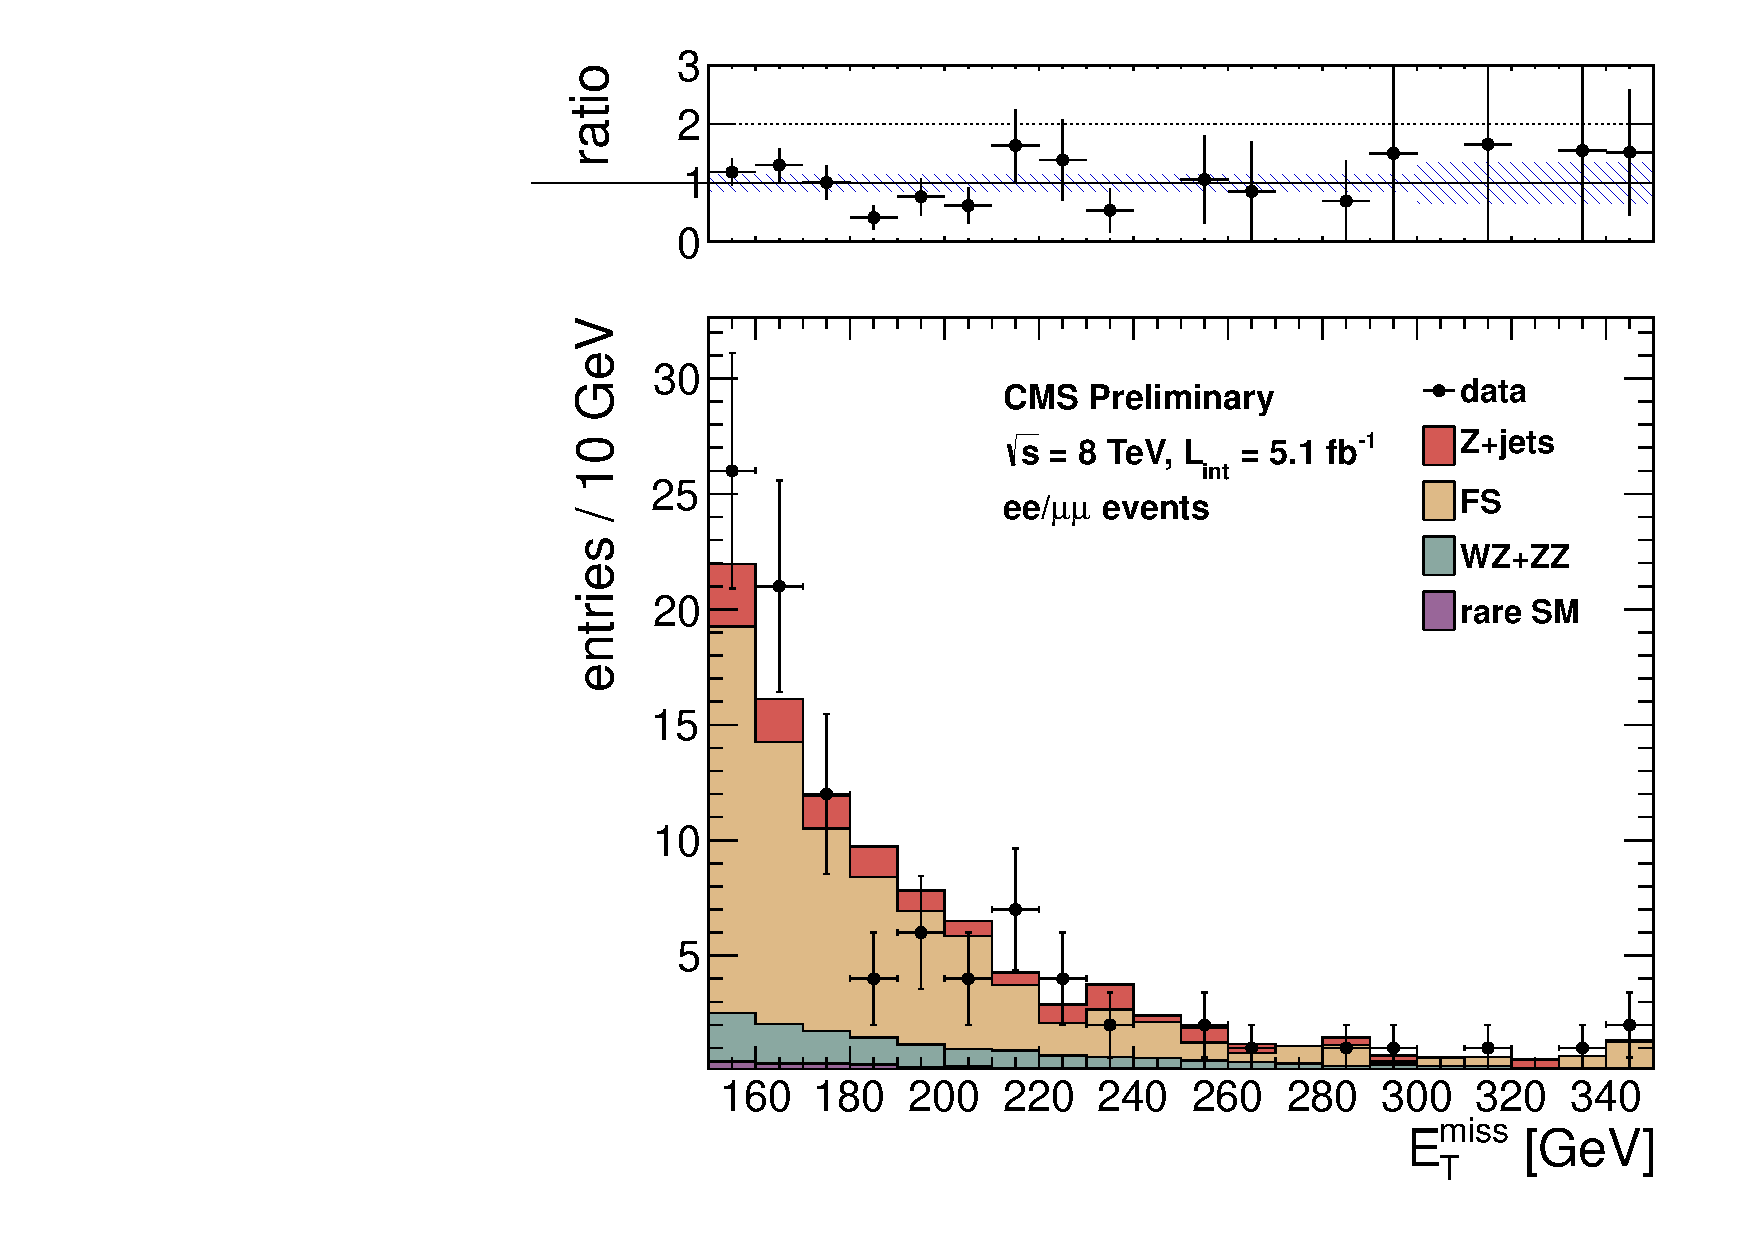
\includegraphics[width=0.48\textwidth]{plots/pfmet_pt40_2012AB_highMet_all_linear.pdf}
\end{tabular}
\caption{\footnotesize Results of for the high \MET\ signal region. 
The results for 5.1 fb$^{-1}$ 2012A+B data are displayed on the left, the results for 4.1 fb$^{-1}$ 2012C data are displayed on the right. 
The observed \MET\ distribution (black points) is compared with the sum of the predicted \MET\
distributions from \zjets, flavor-symmetric backgrounds, WZ+ZZ backgrounds, and rare SM backgrounds. 
The ratio of observed to predicted yields in each bin is
indicated. The error bars indicate the statistical uncertainty in the data and the shaded band indicates the total background uncertainty.
\label{fig:results_highmet}
}
\end{center}
\end{figure}

\begin{table}[htb]
\begin{center}
\footnotesize
\caption{\label{tab:results_highmet}\footnotesize Results for the high \MET\ signal region. 
The results for 5.1 fb$^{-1}$ 2012A+B data are displayed in the top table, the results for 4.1 fb$^{-1}$ 2012C data are displayed in the bottom table. 
The total background is the sum of the \zjets\ background predicted from
the \MET\ templates method (\zjets\ bkg), the flavor-symmetric background predicted from e$\mu$ events (FS bkg), the WZ and ZZ backgrounds predicted from MC
(WZ bkg and ZZ bkg) and the rare SM backgrounds. All uncertainties include both the statistical and systematic components. The Gaussian significance of the deviation between the data 
and total background is indicated for signal regions with at least 20 observed events. }
\begin{tabular}{l|c|c|c|c|c|c}

\hline
\hline

\begin{comment}
Using pfmet out-of-the-box
Using pT > 40 GeV jets, high MET signal region
WZ/ZZ selection : (((((((leptype==0 && (ee==1 || isdata==0))||(leptype==1 && (mm==1 || isdata==0)))&&(ngennu>0))&&(csc==0 && hbhe==1 && hcallaser==1 && ecaltp==1 && trkfail==1 && eebadsc==1 && hbhenew==1))&&(dilmass>81 && dilmass<101))&&(lep1.pt()>20.0 && lep2.pt()>10.0))&&(njets40>=2))&&(ht40>=100.0)
WZ/ZZ weight    : weight * 5.1 * vtxweight * trgeff
Opening ../output/V00-01-04/babylooper_data_ALL_53X_PhotonStitchedTemplate_pfmet_pt40_2012AB_highMet.root
B-veto?   0
K         0.13
ee+mm channels: scale em yield by 0.99
Yields in 0-60 GeV region
data   : 71590
gjets  : 72503.5
OF     : 717.116
WZ     : 63.8074
ZZ     : 7.50741
Rare   : 8.60544
Scaling gjets by : 0.976408
SF events 73711
OF events 11965

ee/#mu#mu events
\end{comment}



                      &   \MET\ $>$ 0 GeV   &  \MET\ $>$ 30 GeV   &  \MET\ $>$ 60 GeV   & \MET\ $>$ 100 GeV   & \MET\ $>$ 150 GeV   & \MET\ $>$ 300 GeV  \\
\hline
        \zjets\ bkg   & 71975 $\pm$ 21593   &  19573 $\pm$ 5873   &    1182 $\pm$ 355   &   70.7 $\pm$ 21.4   &    13.6 $\pm$ 4.2   &     0.4 $\pm$ 0.4  \\
             FS bkg   &    1540 $\pm$ 255   &    1293 $\pm$ 214   &     823 $\pm$ 136   &      313 $\pm$ 52   &   68.6 $\pm$ 11.7   &     2.4 $\pm$ 1.1  \\
             WZ bkg   &  115.9 $\pm$ 81.2   &   91.8 $\pm$ 64.3   &   52.1 $\pm$ 36.5   &   22.4 $\pm$ 15.7   &     8.9 $\pm$ 6.3   &     0.8 $\pm$ 0.8  \\
             ZZ bkg   &   22.6 $\pm$ 11.3   &   20.3 $\pm$ 10.2   &    15.1 $\pm$ 7.6   &     8.8 $\pm$ 4.5   &     4.3 $\pm$ 2.3   &     0.5 $\pm$ 0.5  \\
        rare SM bkg   &   20.6 $\pm$ 10.3   &    17.9 $\pm$ 9.0   &    12.0 $\pm$ 6.1   &     6.3 $\pm$ 3.2   &     2.8 $\pm$ 1.5   &     0.3 $\pm$ 0.3  \\
\hline
          total bkg   & 73674 $\pm$ 21595   &  20996 $\pm$ 5877   &    2084 $\pm$ 382   &      421 $\pm$ 59   &{\bf 98.1 $\pm$ 14.2}&     4.5 $\pm$ 1.5  \\
               data   &             73711   &             20601   &              2121   &               446   &          {\bf 95 }  &                 4  \\
       significance   &       0.0$\sigma$   &      -0.1$\sigma$   &       0.1$\sigma$   &       0.4$\sigma$   &{\bf -0.2$\sigma$ }  &                    \\

\hline
\hline

\begin{comment}
Using pfmet out-of-the-box
Using pT > 40 GeV jets, high MET signal region
WZ/ZZ selection : (((((((leptype==0 && (ee==1 || isdata==0))||(leptype==1 && (mm==1 || isdata==0)))&&(ngennu>0))&&(csc==0 && hbhe==1 && hcallaser==1 && ecaltp==1 && trkfail==1 && eebadsc==1 && hbhenew==1))&&(dilmass>81 && dilmass<101))&&(lep1.pt()>20.0 && lep2.pt()>10.0))&&(njets40>=2))&&(ht40>=100.0)
WZ/ZZ weight    : weight * 4.1 * vtxweight * trgeff
Opening ../output/V00-01-04/babylooper_data_ALL_53X_PhotonStitchedTemplate_pfmet_pt40_2012C_highMet.root
B-veto?   0
K         0.13
ee+mm channels: scale em yield by 0.99
Yields in 0-60 GeV region
data   : 56788
gjets  : 57414.8
OF     : 557.657
WZ     : 51.2961
ZZ     : 6.03537
Rare   : 6.9181
Scaling gjets by : 0.978251
SF events 58478
OF events 9373

ee/#mu#mu events
\end{comment}

                      &   \MET\ $>$ 0 GeV   &  \MET\ $>$ 30 GeV   &  \MET\ $>$ 60 GeV   & \MET\ $>$ 100 GeV   & \MET\ $>$ 150 GeV   & \MET\ $>$ 300 GeV  \\
\hline
        \zjets\ bkg   & 57206 $\pm$ 17163   &  15965 $\pm$ 4790   &    1040 $\pm$ 313   &   68.3 $\pm$ 21.5   &    17.5 $\pm$ 6.0   &     1.4 $\pm$ 0.4  \\
             FS bkg   &    1206 $\pm$ 200   &    1015 $\pm$ 168   &     649 $\pm$ 108   &      244 $\pm$ 41   &    48.1 $\pm$ 8.3   &     1.3 $\pm$ 0.6  \\
             WZ bkg   &   93.2 $\pm$ 65.3   &   73.8 $\pm$ 51.7   &   41.9 $\pm$ 29.4   &   18.0 $\pm$ 12.7   &     7.1 $\pm$ 5.1   &     0.7 $\pm$ 0.7  \\
             ZZ bkg   &    18.2 $\pm$ 9.1   &    16.3 $\pm$ 8.2   &    12.1 $\pm$ 6.1   &     7.1 $\pm$ 3.6   &     3.4 $\pm$ 1.8   &     0.4 $\pm$ 0.4  \\
        rare SM bkg   &    16.6 $\pm$ 8.3   &    14.4 $\pm$ 7.2   &     9.7 $\pm$ 4.9   &     5.1 $\pm$ 2.6   &     2.3 $\pm$ 1.2   &     0.3 $\pm$ 0.3  \\
\hline
          total bkg   & 58541 $\pm$ 17164   &  17084 $\pm$ 4793   &    1753 $\pm$ 332   &      343 $\pm$ 48   &{\bf 78.4 $\pm$ 11.7}&     4.0 $\pm$ 1.1  \\
               data   &             58478   &             16494   &              1690   &               321   &        {\bf 72 }    &                 1  \\
       significance   &      -0.0$\sigma$   &      -0.1$\sigma$   &      -0.2$\sigma$   &      -0.4$\sigma$   &{\bf -0.4$\sigma$}   &                    \\

\hline
\hline

\end{tabular}
\end{center}
\end{table}


\clearpage



\begin{figure}[!h]
\begin{center}
\begin{tabular}{cc}
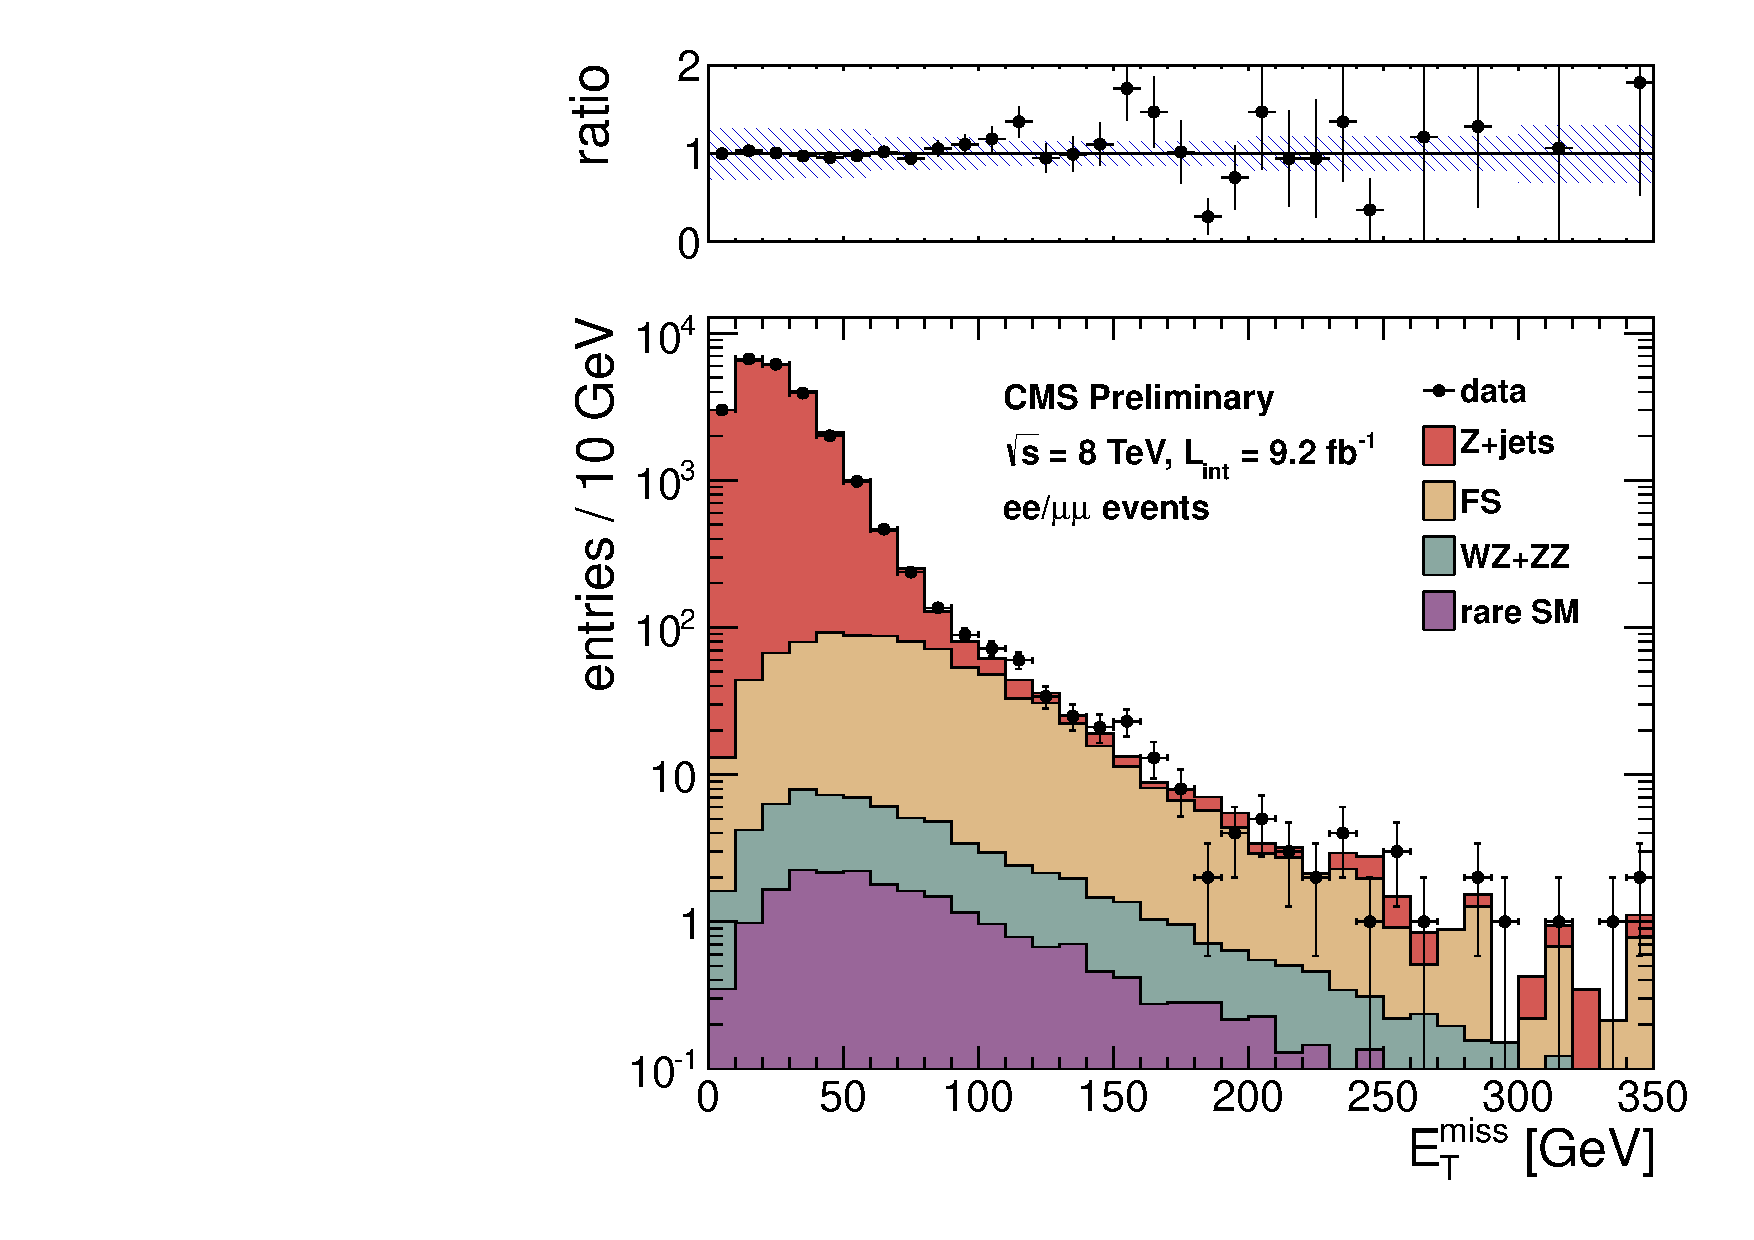
\includegraphics[width=0.45\textwidth]{plots/pfmet_pt40_lowMet_all.pdf}
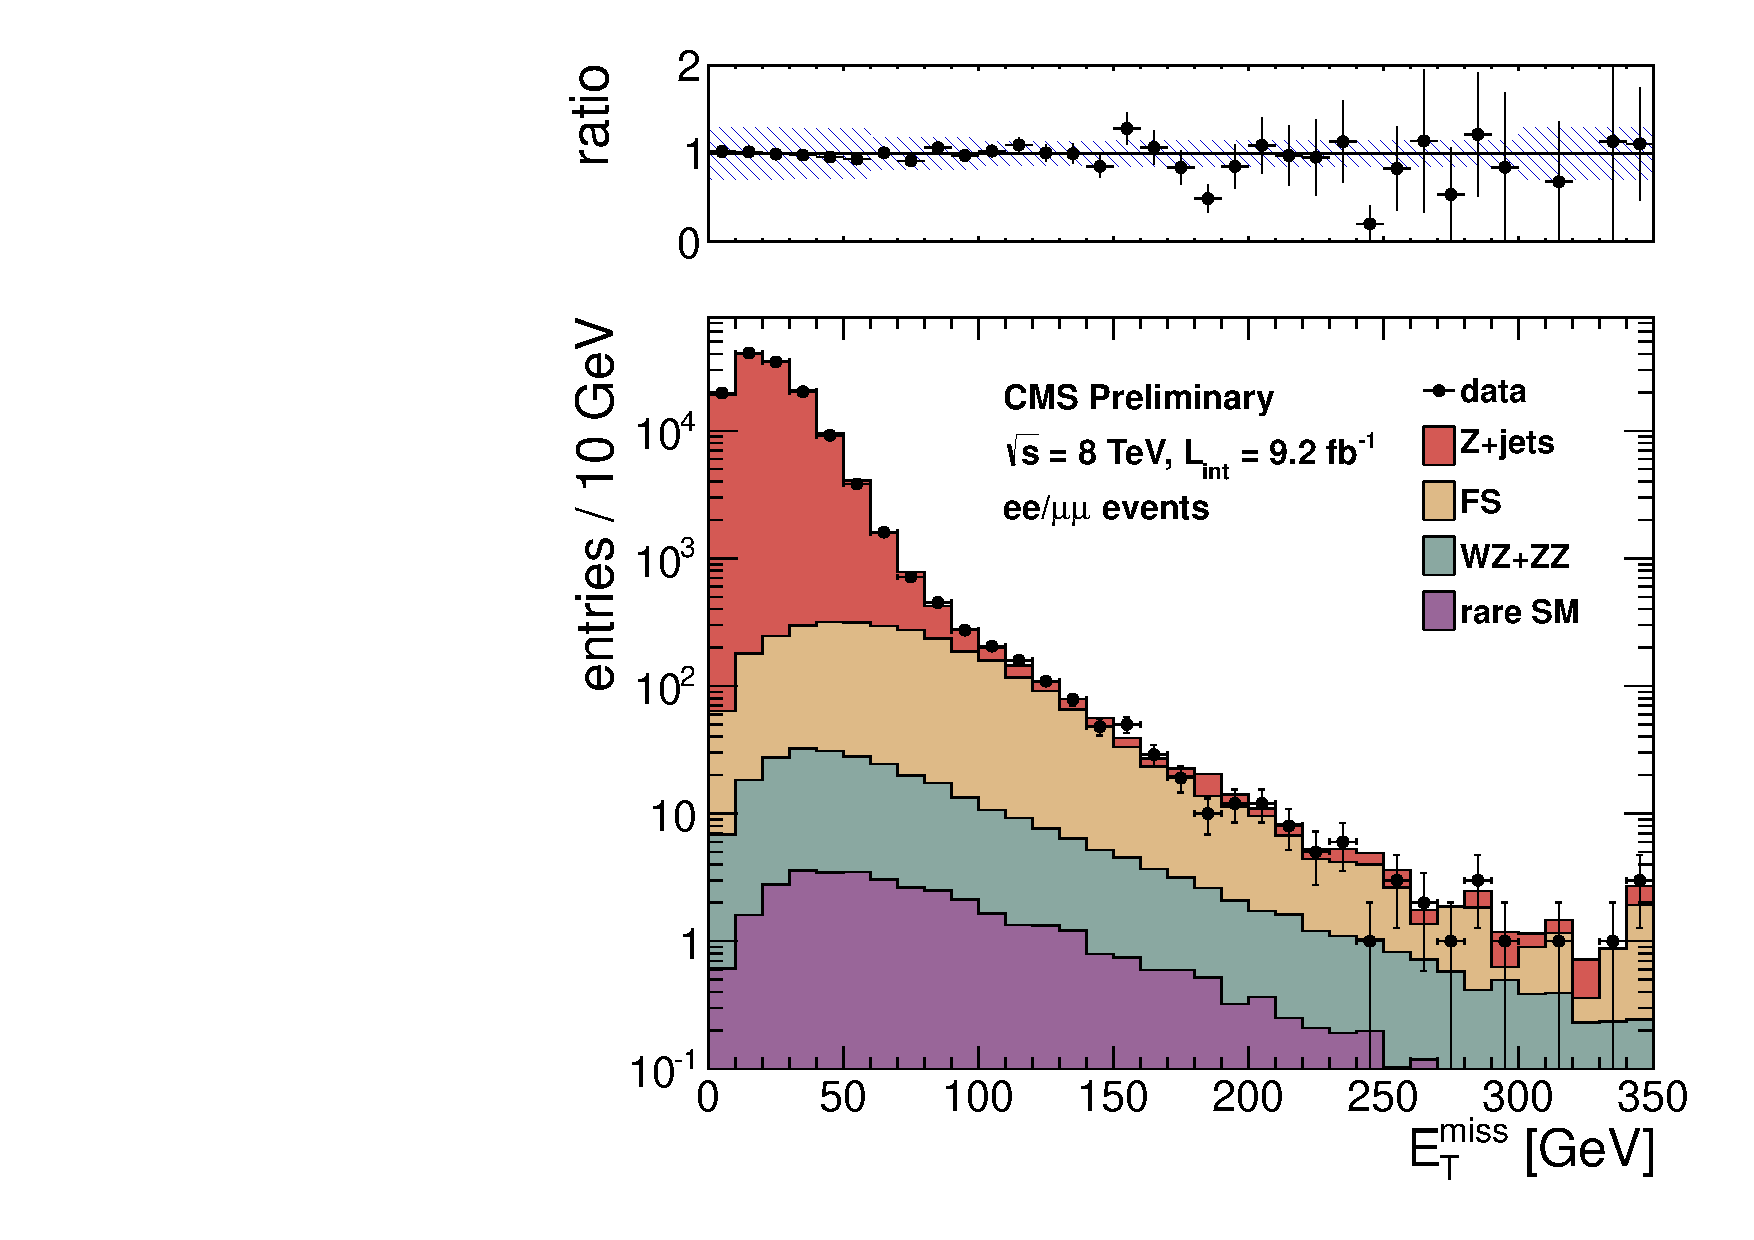
\includegraphics[width=0.45\textwidth]{plots/pfmet_pt40_highMet_all.pdf}
%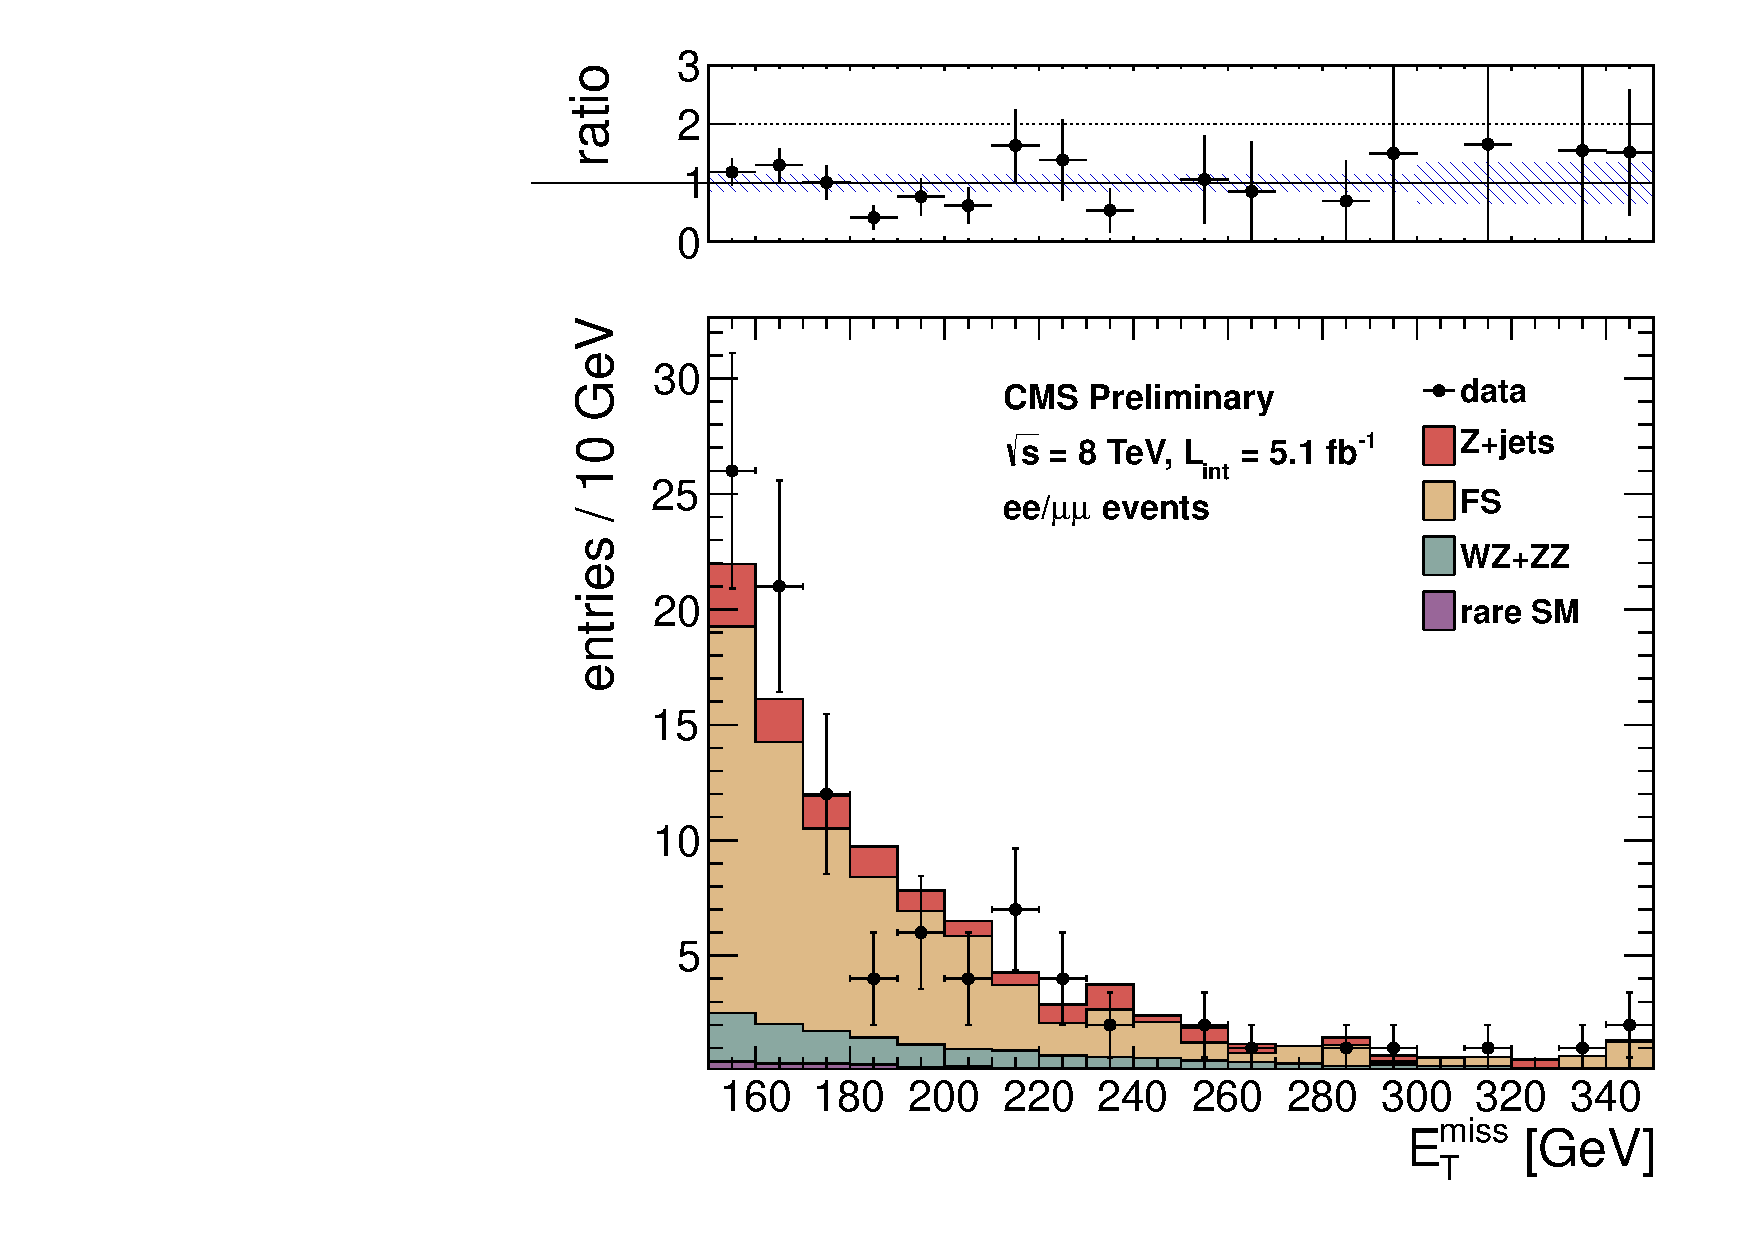
\includegraphics[width=0.48\textwidth]{plots/pfmet_pt40_2012AB_highMet_all_linear.pdf}
\end{tabular}
\caption{\footnotesize Results of for the low \MET\ (left) and high \MET\ (right) signal regions for the full 9.2 fb$^{-1}$ sample.
The observed \MET\ distribution (black points) is compared with the sum of the predicted \MET\
distributions from \zjets, flavor-symmetric backgrounds, WZ+ZZ backgrounds, and rare SM backgrounds. 
The ratio of observed to predicted yields in each bin is
indicated. The error bars indicate the statistical uncertainty in the data and the shaded band indicates the total background uncertainty.
\label{fig:results_fulledge}
}
\end{center}
\end{figure}

\begin{table}[htb]
\begin{center}
\footnotesize
\caption{\label{tab:results_edgefull}\footnotesize Results for the low \MET\ signal region (top table) and high \MET\ signal region (bottom table). 
The total background is the sum of the \zjets\ background predicted from
the \MET\ templates method (\zjets\ bkg), the flavor-symmetric background predicted from e$\mu$ events (FS bkg), the WZ and ZZ backgrounds predicted from MC
(WZ bkg and ZZ bkg) and the rare SM backgrounds. All uncertainties include both the statistical and systematic components. The Gaussian significance of the deviation between the data 
and total background is indicated for signal regions with at least 20 observed events. }
\begin{tabular}{l|c|c|c|c|c|c}

\hline
\hline

\begin{comment}
Using pfmet out-of-the-box
Using pT > 40 GeV jets, low MET signal region
WZ/ZZ selection : ((((((leptype==0 && (ee==1 || isdata==0))||(leptype==1 && (mm==1 || isdata==0)))&&(ngennu>0))&&(csc==0 && hbhe==1 && hcallaser==1 && ecaltp==1 && trkfail==1 && eebadsc==1 && hbhenew==1))&&(dilmass>81 && dilmass<101))&&(lep1.pt()>20.0 && lep2.pt()>20.0))&&(njets40>=3)
WZ/ZZ weight    : weight * 9.2 * vtxweight * trgeff
Opening ../output/V00-01-04/babylooper_data_ALL_53X_PhotonStitchedTemplate_pfmet_pt40_lowMet.root
B-veto?   0
K         0.14
ee+mm channels: scale em yield by 0.99
Yields in 0-60 GeV region
data   : 22782
gjets  : 23298
OF     : 350.242
WZ     : 22.2641
ZZ     : 2.36791
Rare   : 9.60548
Scaling gjets by : 0.96135
SF events 23999
OF events 5826

ee/#mu#mu events
\end{comment}
                      &   \MET\ $>$ 0 GeV   &  \MET\ $>$ 30 GeV   &  \MET\ $>$ 60 GeV   & \MET\ $>$ 100 GeV   & \MET\ $>$ 200 GeV   & \MET\ $>$ 300 GeV  \\
\hline
        \zjets\ bkg   &  23072 $\pm$ 6922   &   7566 $\pm$ 2270   &     674 $\pm$ 203   &   47.9 $\pm$ 14.6   &     4.7 $\pm$ 1.6   &     1.1 $\pm$ 0.4  \\
             FS bkg   &     807 $\pm$ 126   &     695 $\pm$ 108   &      457 $\pm$ 71   &      184 $\pm$ 29   &    14.1 $\pm$ 3.4   &     1.5 $\pm$ 0.9  \\
             WZ bkg   &   43.5 $\pm$ 30.5   &   35.1 $\pm$ 24.6   &   21.3 $\pm$ 14.9   &    10.0 $\pm$ 7.1   &     1.9 $\pm$ 1.7   &     0.4 $\pm$ 0.4  \\
             ZZ bkg   &     7.8 $\pm$ 3.9   &     7.0 $\pm$ 3.6   &     5.4 $\pm$ 2.8   &     3.3 $\pm$ 1.8   &     0.9 $\pm$ 0.8   &     0.2 $\pm$ 0.2  \\
        rare SM bkg   &   22.0 $\pm$ 11.0   &    19.0 $\pm$ 9.6   &    12.4 $\pm$ 6.3   &     6.3 $\pm$ 3.3   &     1.3 $\pm$ 1.1   &     0.3 $\pm$ 0.3  \\
\hline
          total bkg   &  23952 $\pm$ 6923   &   8323 $\pm$ 2273   &    1170 $\pm$ 216   &{\bf  251 $\pm$ 33}  &    22.8 $\pm$ 4.4   &     3.5 $\pm$ 1.1  \\
               data   &             23999   &              8134   &              1217   &{\bf           288}  &                26   &                 4  \\
       significance   &       0.0$\sigma$   &      -0.1$\sigma$   &       0.2$\sigma$   &{\bf   1.0$\sigma$}  &       0.5$\sigma$   &                    \\
\hline
\hline

\begin{comment}
Using pfmet out-of-the-box
Using pT > 40 GeV jets, high MET signal region
WZ/ZZ selection : (((((((leptype==0 && (ee==1 || isdata==0))||(leptype==1 && (mm==1 || isdata==0)))&&(ngennu>0))&&(csc==0 && hbhe==1 && hcallaser==1 && ecaltp==1 && trkfail==1 && eebadsc==1 && hbhenew==1))&&(dilmass>81 && dilmass<101))&&(lep1.pt()>20.0 && lep2.pt()>10.0))&&(njets40>=2))&&(ht40>=100.0)
WZ/ZZ weight    : weight * 9.2 * vtxweight * trgeff
Opening ../output/V00-01-04/babylooper_data_ALL_53X_PhotonStitchedTemplate_pfmet_pt40_highMet.root
B-veto?   0
K         0.13
ee+mm channels: scale em yield by 0.99
Yields in 0-60 GeV region
data   : 128378
gjets  : 129908
OF     : 1274.77
WZ     : 115.104
ZZ     : 13.5428
Rare   : 15.5235
Scaling gjets by : 0.977303
SF events 132189
OF events 21338

ee/#mu#mu events
\end{comment}

                      &   \MET\ $>$ 0 GeV   &  \MET\ $>$ 30 GeV   &  \MET\ $>$ 60 GeV   & \MET\ $>$ 100 GeV   & \MET\ $>$ 150 GeV   & \MET\ $>$ 300 GeV  \\
\hline
        \zjets\ bkg   &129184 $\pm$ 38756   & 35565 $\pm$ 10670   &    2225 $\pm$ 668   &      140 $\pm$ 43   &   31.6 $\pm$ 10.1   &     1.7 $\pm$ 0.6  \\
             FS bkg   &    2746 $\pm$ 454   &    2308 $\pm$ 382   &    1471 $\pm$ 243   &      557 $\pm$ 92   &      117 $\pm$ 20   &     3.7 $\pm$ 1.6  \\
             WZ bkg   & 209.2 $\pm$ 146.4   & 165.6 $\pm$ 115.9   &   94.1 $\pm$ 65.9   &   40.5 $\pm$ 28.4   &   16.0 $\pm$ 11.3   &     1.5 $\pm$ 1.5  \\
             ZZ bkg   &   40.8 $\pm$ 20.4   &   36.6 $\pm$ 18.4   &   27.2 $\pm$ 13.7   &    16.0 $\pm$ 8.1   &     7.7 $\pm$ 4.1   &     0.9 $\pm$ 0.9  \\
        rare SM bkg   &   37.2 $\pm$ 18.7   &   32.2 $\pm$ 16.2   &   21.7 $\pm$ 10.9   &    11.4 $\pm$ 5.8   &     5.1 $\pm$ 2.8   &     0.6 $\pm$ 0.6  \\
\hline
          total bkg   &132217 $\pm$ 38759   & 38108 $\pm$ 10678   &    3839 $\pm$ 714   &     765 $\pm$ 106   &{\bf 177 $\pm$ 25}   &     8.4 $\pm$ 2.5  \\
               data   &            132189   &             37095   &              3811   &               767   &{\bf          167}   &                 5  \\
       significance   &      -0.0$\sigma$   &      -0.1$\sigma$   &      -0.0$\sigma$   &       0.0$\sigma$   &{\bf -0.4$\sigma$}   &                    \\

\hline
\hline

\end{tabular}
\end{center}
\end{table}




\clearpage


\begin{figure}[t]
\begin{center}
\begin{tabular}{cc}
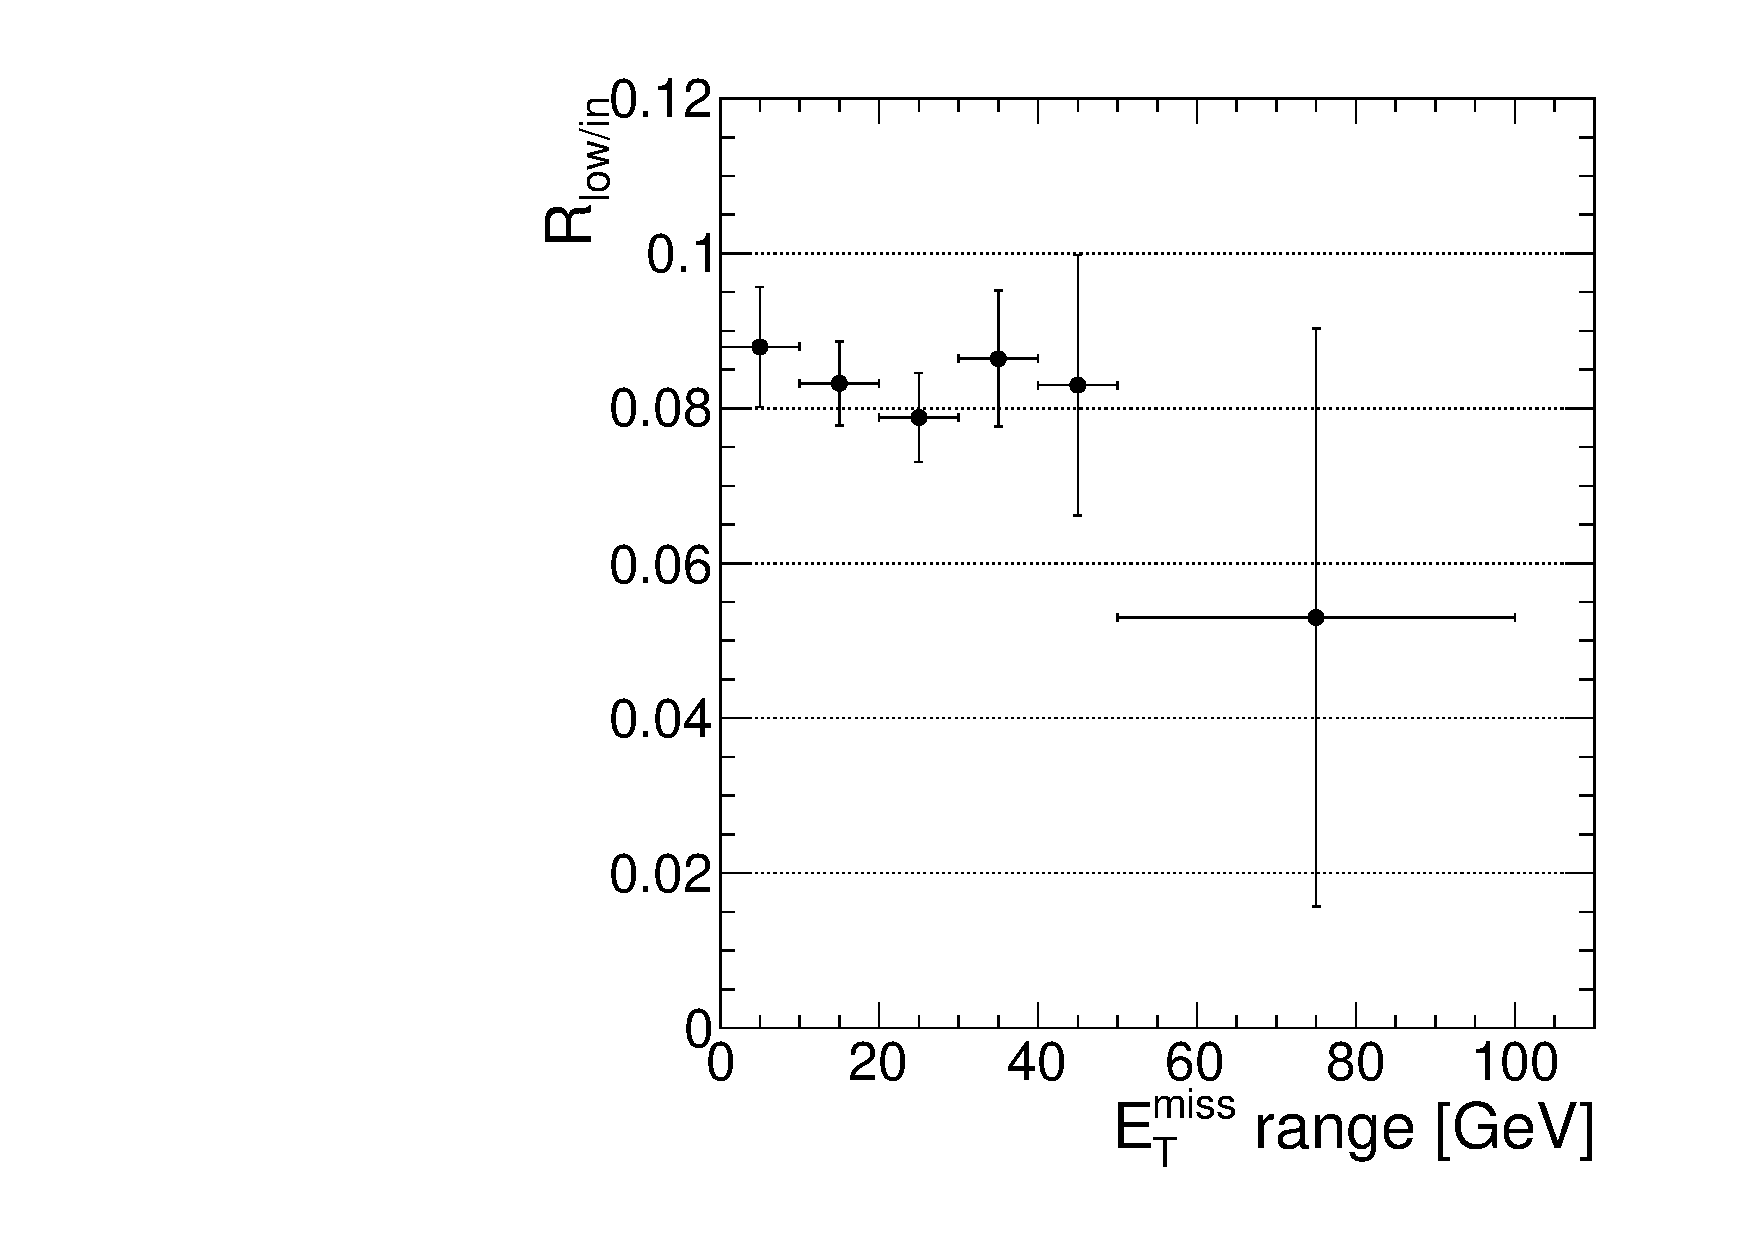
\includegraphics[width=0.4\textwidth]{plots/Routin_lowmet.pdf} &
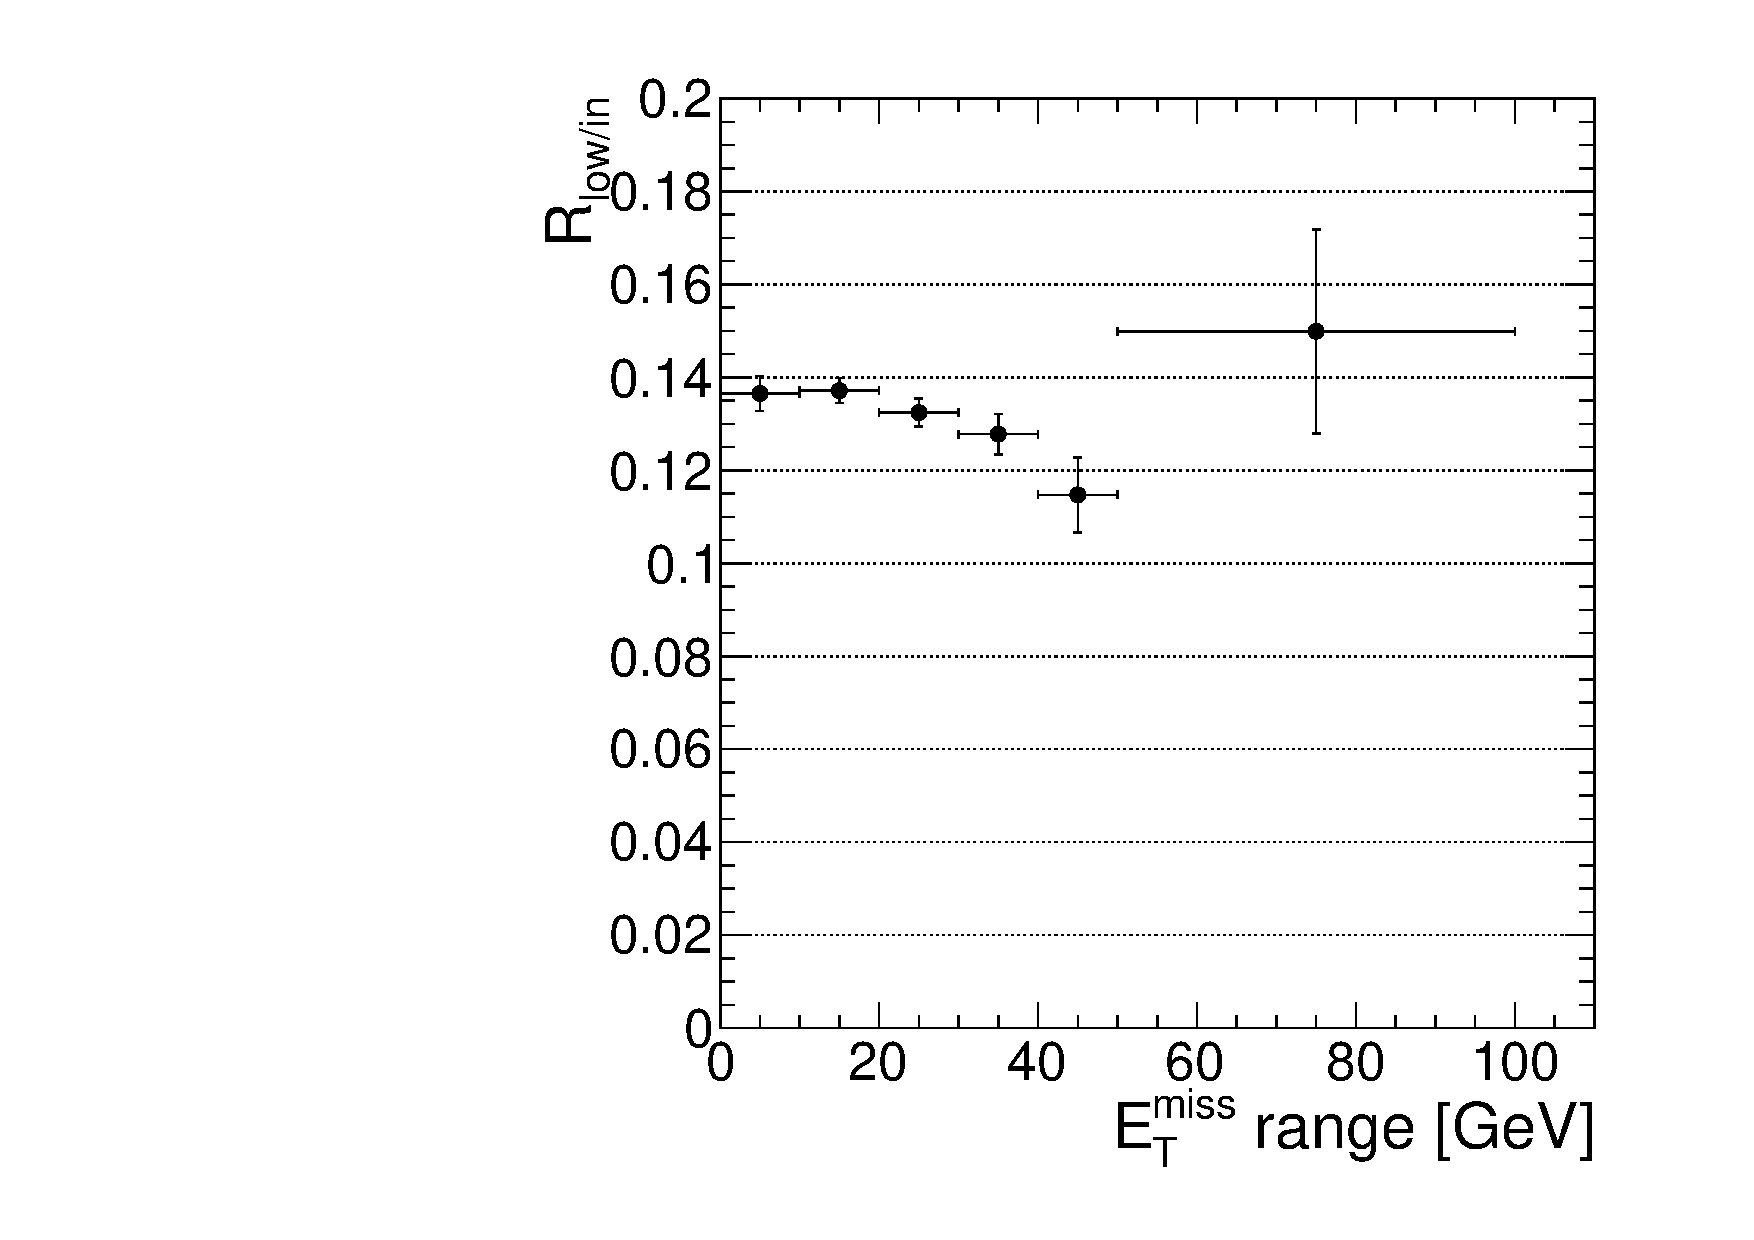
\includegraphics[width=0.4\textwidth]{plots/Routin_highMET.pdf} \\
\end{tabular}
\caption{\label{fig:Routin}
The ratio $R_{low/in}$ of low mass ($15<m_{\ell\ell}<70$ GeV) to on-Z ($81<m_{\ell\ell}<101$ GeV) events, as a function of
the \MET\ requirement. The left plot corresponds to the low \MET\ signal region (2 \pt\ $>$ 20 GeV leptons with at least 3 jets),
the right plot corresponds to the high \MET\ signal region (\pt\ $>$ (20,10) GeV leptons with at least 2 jets). 
}
\end{center}
\end{figure}

Given a prediction for the Z background in the Z mass window, we can extrapolate to estimate the low mass $\gamma^*$/Z contribution.
We extract the ratio $R_{low/in}$ of low-mass  to on-shell Z events from data,
correcting for the contribution from flavor-symmetric backgrounds, according to:

\begin{equation}
R_{low/in} = (N_{SF}^{low}-N_{OF}^{low})/(N_{SF}^{in}-N_{OF}^{in}).
\end{equation}

Here SF and OF refer to the same-flavor and opposite-flavor data yields in the ``low'' ($15<m_{\ell\ell}<70$ GeV) and ``in'' 
($81<m_{\ell\ell}<101$ GeV) dilepton mass regions. To predict the low-mass $\gamma^*$/Z contribution, we scale the total predicted
Z background by this quantity, which is displayed in Fig.~\ref{fig:Routin}. Here we measure $R_{low/in}$ in several \MET\ regions,
and assess the uncertainty based on the variation with respect to \MET. 
Based on this plot we choose $R_{low/in}=0.08\pm0.02$ for the low \MET\ signal region and $R_{low/in}=0.13\pm0.03$ for the high \MET\ region.

\clearpage

We find the following results for the first 5.1 fb$^{-1}$. For the low \MET\ signal region, the total predicted Z background in the Z mass region is $39\pm9.6$ 
(sum of the \zjets, WZ+ZZ, and rare SM backgrounds from Table~\ref{tab:results_lowmet}, \MET\ $>$ 100 GeV region), 
resulting in a $\gamma^*$/Z prediction of $3.1\pm1.1$ events. 
For the high \MET\ signal region, the total predicted Z background in the Z mass region is $30\pm8.1$ 
(sum of the \zjets, WZ+ZZ, and rare SM backgrounds from Table~\ref{tab:results_highmet}, \MET\ $>$ 150 GeV region), 
resulting in a $\gamma^*$/Z prediction of $3.8\pm1.4$ events. 
Hence we summarize the 5.1 fb$^{-1}$ results as:

\begin{itemize}
\item Low \MET\ signal region
\begin{itemize}
  \item Total predicted background in Z mass region: $138\pm18$ events
  \item Total observed yield in Z mass region: 175 events ($+1.6\sigma$)
  \item Low-mass $\gamma^*$/Z prediction: $3.1\pm1.1$ events
\end{itemize}
\item High \MET\ signal region
\begin{itemize}
  \item Total predicted background in Z mass region: $98\pm14$ events
  \item Total observed yield in Z mass region: 95 events ($-0.2\sigma$)
  \item Low-mass $\gamma^*$/Z prediction: $3.8\pm1.4$ events
\end{itemize}
\end{itemize}

We find the following results for the full 9.2 fb$^{-1}$. For the low \MET\ signal region, the total predicted Z background in the Z mass region is $68\pm17$ 
(sum of the \zjets, WZ+ZZ, and rare SM backgrounds from Table~\ref{tab:results_edgefull}, \MET\ $>$ 100 GeV region), 
resulting in a $\gamma^*$/Z prediction of $5.4\pm1.9$ events. 
For the high \MET\ signal region, the total predicted Z background in the Z mass region is $60\pm16$ 
(sum of the \zjets, WZ+ZZ, and rare SM backgrounds from Table~\ref{tab:results_edgefull}, \MET\ $>$ 150 GeV region), 
resulting in a $\gamma^*$/Z prediction of $7.9\pm2.7$ events. 
Hence we summarize the 9.2 fb$^{-1}$ results as:

\begin{itemize}
\item Low \MET\ signal region
\begin{itemize}
  \item Total predicted background in Z mass region: $251\pm33$ events
  \item Total observed yield in Z mass region: 288 events ($+1.0\sigma$)
  \item Low-mass $\gamma^*$/Z prediction: $5.4\pm1.9$ events
\end{itemize}
\item High \MET\ signal region
\begin{itemize}
  \item Total predicted background in Z mass region: $177\pm25$ events
  \item Total observed yield in Z mass region: 167 events ($-0.4\sigma$)
  \item Low-mass $\gamma^*$/Z prediction: $7.9\pm2.7$ events
\end{itemize}
\end{itemize}

\clearpage

\subsection{Cross-check with single lepton triggers}
\label{sec:edge_triggers}

The nominal ``edge analysis'' is performed with dilepton triggers. An excess of SF vs. OF events may thus be observed if there
were some inefficiency for the e$\mu$ triggers used in this analysis. In this section we provide a cross-check of the nominal
analysis by including events collected with single lepton triggers. The relevant triggers are:

\begin{itemize}

\item ee channel
\begin{itemize}
\item dilepton: {\footnotesize \verb=HLT_Ele17_CaloIdT_CaloIsoVL_TrkIdVL_TrkIsoVL_Ele8_CaloIdT_CaloIsoVL_TrkIdVL_TrkIsoVL=}
\item single lepton: \verb=HLT_Ele27_WP80=
\end{itemize}

\item $\mu\mu$ channel
\begin{itemize}
\item dilepton: \verb=HLT_Mu17_Mu8= OR \verb=HLT_Mu17_TkMu8=
\item single lepton: \verb=HLT_IsoMu24= OR \verb=HLT_IsoMu24_eta2p1=
\end{itemize}

\item $e\mu$ channel
\begin{itemize}
\item dilepton: \verb=HLT_MuX_EleY_CaloIdT_CaloIsoVL_TrkIdVL_TrkIsoVL= (X,Y=17,8 OR 8,17)
\item single lepton: \verb=HLT_Ele27_WP80= OR \verb=HLT_IsoMu24= OR \verb=HLT_IsoMu24_eta2p1=
\end{itemize}

\end{itemize}


In the nominal analysis based on dilepton triggers only, an ee event is required to satisfy the ee dilepton trigger, a $\mu\mu$ event is required to
satisfy one of the two $\mu\mu$ dilepton triggers, and an e$\mu$ event is required to satisfy one of the two e$\mu$ dilepton triggers. Here we compare
the results obtained from the nominal dilepton triggers with those obtained by requiring an OR of the dilepton and single lepton triggers. In this cross-check,
an ee event is required to satisfy the ee dilepton trigger OR single electron trigger, a $\mu\mu$ event is required to
satisfy one of the two $\mu\mu$ dilepton triggers OR one of the two single muon triggers, and an e$\mu$ event is required to satisfy one of the two e$\mu$ dilepton triggers
OR the single electron trigger OR the single muon trigger. The results are summarized in Table~\ref{tab:triggers}. Including the single lepton triggers increases
the yields in the ee, $\mu\mu$ and e$\mu$ final states by (1--7)\%, and does not significantly alter the excess of SF vs. OF data yields.

\begin{table}[htb]
\begin{center}
\footnotesize
\caption{\label{tab:triggers} Summary of results comparing dilepton vs. dilepton OR single lepton triggers, for 5.1 fb$^{-1}$,
in the low \MET\ and high \MET\ signal regions (SR). The ratio of the dilepton OR single lepton yield to the dilepton only yield
is indicated, along with the excess of SF w.r.t. OF events.}
\begin{tabular}{l|c|c|c|c}
\hline
\hline
Region & $N_{\rm{ee}}$ & $N_{\mu\mu}$ & $N_{\rm{e}\mu}$ & $N_{\rm{ee}}+N_{\mu\mu}-N_{\rm{e}\mu}$ \\
\hline
\hline
Low \MET\ SR and $20<m_{\ell\ell}<70$~GeV & & & \\
dilepton (nominal)        & 106 & 153 & 189 & 70 $\pm$ 21.2 (stat)  \\
dilepton OR single lepton & 112 & 155 & 199 & 68 $\pm$ 21.6 (stat)  \\
ratio                     & 1.06 & 1.01 & 1.05 &                    \\
\hline
\hline
Low \MET\ SR and $m_{\ell\ell}>20$~GeV & & & \\
dilepton (nominal)        & 357 & 517 & 693 & 181 $\pm$ 39.6 (stat)  \\
dilepton OR single lepton & 368 & 534 & 739 & 163 $\pm$ 40.5 (stat)  \\
ratio                     & 1.03 & 1.03 & 1.07 &                     \\
\hline
\hline
High \MET\ SR and $15<m_{\ell\ell}<70$~GeV & & & \\
dilepton (nominal)        & 89 & 157 & 187 & 59 $\pm$ 20.8 (stat)  \\
dilepton OR single lepton & 93 & 160 & 197 & 56 $\pm$ 21.2 (stat)  \\
ratio                     & 1.04 & 1.02 & 1.05 &                   \\
\hline
\hline
High \MET\ SR and $m_{\ell\ell}>15$~GeV & & & \\
dilepton (nominal)        & 258 & 380 & 527 & 111 $\pm$ 34.1 (stat)  \\
dilepton OR single lepton & 271 & 386 & 553 & 104 $\pm$ 34.8 (stat)  \\
ratio                     & 1.05 & 1.02 & 1.05 &                     \\
\hline
\hline
\end{tabular}
\end{center}
\end{table}

\clearpage

Next, we compare the results obtained with the dilepton triggers to results obtained with single lepton triggers only. Since the single electron (single muon)
triggers have \pt\ thresholds of 27 (24) GeV, we use a dilepton \pt\ $>$ (30,20) selection. The results are summarized in Table~\ref{tab:trigger2}.
Switching from dilepton to single lepton triggers alters the yields by (-2--5)\%, and does not significantly alter the excess of SF vs. OF data yields.

\begin{table}[htb]
\begin{center}
\footnotesize
\caption{\label{tab:trigger2} Summary of results comparing dilepton vs. single lepton triggers (with a dilepton \pt\ $>$ (30,20) GeV selection, 
for 5.1 fb$^{-1}$, in the low \MET\ and high \MET\ signal regions (SR). The ratio of the single lepton trigger yield to the dilepton trigger yield
is indicated, along with the excess of SF w.r.t. OF events.}
\begin{tabular}{l|c|c|c|c}
\hline
\hline
Region & $N_{\rm{ee}}$ & $N_{\mu\mu}$ & $N_{\rm{e}\mu}$ & $N_{\rm{ee}}+N_{\mu\mu}-N_{\rm{e}\mu}$ \\
\hline
\hline
Low \MET\ SR and $20<m_{\ell\ell}<70$~GeV & & & \\
dilepton                  & 95 & 135 & 169 & 61 $\pm$ 20.0 (stat)  \\
single lepton             & 93 & 134 & 172 & 55 $\pm$ 20.0 (stat)  \\
ratio                     & 0.98 & 0.99 & 1.02 &                   \\
\hline
\hline
Low \MET\ SR and $m_{\ell\ell}>20$~GeV & & & \\
dilepton                  & 345 & 497 & 669 & 173 $\pm$ 38.9 (stat)  \\
single lepton             & 346 & 499 & 700 & 145 $\pm$ 39.3 (stat)  \\
ratio                     & 1.00 & 1.00 & 1.05 &                     \\
\hline
\hline
High \MET\ SR and $15<m_{\ell\ell}<70$~GeV & & & \\
dilepton                  & 48 & 72 & 79 & 41 $\pm$ 14.1 (stat)  \\
single lepton             & 47 & 72 & 81 & 38 $\pm$ 14.1 (stat)  \\
ratio                     & 0.98 & 1.00 & 1.03 &             \\
\hline
\hline
High \MET\ SR and $m_{\ell\ell}>15$~GeV & & & \\
dilepton                  & 197 & 270 & 367 & 100 $\pm$ 28.9 (stat)  \\
single lepton             & 200 & 269 & 377 & 92 $\pm$ 29.1 (stat)  \\
ratio                     & 1.02 & 1.00 & 1.03 &             \\
\hline
\hline
\end{tabular}
\end{center}
\end{table}


